\documentclass[a4paper, british]{memoir}

\usepackage{style}           % Custom style
\usepackage{masterfrontpage} % Front page
\usepackage{kantlipsum}      % Dummy text
%\usepackage[utf8]{inputenc}
\usepackage{amsmath}
\usepackage{bbold}
\usepackage{algorithm}
\usepackage[noend]{algpseudocode}
\algnewcommand{\algorithmicand}{\textbf{ and }}
\algnewcommand{\algorithmicor}{\textbf{ or }}
\algnewcommand{\OR}{\algorithmicor}
\algnewcommand{\AND}{\algorithmicand}
\usepackage{amsthm}
\usepackage{geometry}[margins = 1in]
\renewcommand{\baselinestretch}{1.5}
\theoremstyle{definition}
\usepackage{algorithm}
%\usepackage[round]{natbib}
\usepackage[acronym]{glossaries}
\usepackage{todonotes}
\usepackage{mathtools}
%\usepackage{natbib}
\usepackage[mathscr]{euscript}
\let\euscr\mathscr \let\mathscr\relax% just so we can load this and rsfs
\usepackage[scr]{rsfso}
\newcommand{\powerset}{\raisebox{.15\baselineskip}{\Large\ensuremath{\wp}}}
%\loadglsentries{glossary}
%\usepackage[backend=biber,citestyle=numeric]{biblatex}
\addbibresource{bibliography.bib}
\title{\textsc{Scalable Markov Chain Monte Carlo by subsampling methods}}
\author{\textsc{Oda Johanne Kristensen}}
\date{}
\usepackage{listings}
\title{Title}
\subtitle{Optional Subtitle}
\author{Author}

\includeonly
{
    sections/introduction,
    sections/chapter2, 
    sections/chapter3, 
    sections/chapter4
    %sections/chapter5
}

\begin{document}

    \frontmatter        % Folios in Roman numerals, unnumbered chapters.

    %\masterfrontpage

    %\chapter{Abstract}
\kant[1] % Dummy text
\todo[inline]{Add new section about results in \cref{sec:fourth}.}
   % \chapter{Acknowledgements}

\kant[2] % Dummy text
\todo[noline]{Rewrite this.}
\kant[3] % Dummy text

    \cleartorecto
    \tableofcontents    % Or \tableofcontents*
    \cleartorecto
    \listoffigures      % Or \listoffigures*
    \cleartorecto
    %\listoftables       % Or \listoftables*

    \mainmatter         % Folios in Arabic numerals, numbered chapters.

% \chapter{Introduction}
\label{sec:intro}

\section{Notation}
$\theta$ : Model parameter \\
$\mathbf{X}$ : \\
$\mathbf{x}$: explanatory variable \\
$\mathbf{Y}$: \\
$\mathbf{y}$: response \\
$\mathbf{z}:$ auxilliary variables \\ 
$n$: indexes the data \\ 
$i$: indexes the simulated parameters \\
$p\left(\cdot\right):$ A probability mass function or a probability density function  Its arguments indicate whether it is a prior, posterior or other.  \\
$g\left(\cdot\mid \theta \right):$ proposal distribution MCMC

\section{Bayesian statistics}\label{sec:bayesian}
Traditionally, statistics has been divided into two schools, frequentist statistics and Bayesian statistics. 
There are many interpretations of the difference in philosophy between these two schools, which we will not go into very deeply here, but statisticians in favour of using Bayesian methods rather than frequentist, argue that one limitation of frequentist methods is that inference is not conditional on the observed data \cite{Wagenmakers}. 
In the frequentist approach, the parameter $\theta$ is thought of as fixed, but unknown, meaning that there exists some true $\theta$ that can describe the model, and inference about this parameter is only based on the available data from that population. 
In Bayesian statistics on the other hand, $\theta$ is represented by a probability distribution. Using a probability distribution to represent $\theta$, allows us to express that there is an uncertainty in the true value of $\theta$. In Bayesian inference there are two distributions that represent $\theta$.  
Before any data has been considered, a belief, or knowledge about $\theta$ is represented by what we call the prior\cite{SI}. The prior is  a probability distribution, which can be flat if we have very little knowledge of $\theta$ or it may be more informative in a certain area of the distribution if there is a lot of prior knowledge. 
\todo{Sjekk denne referansen}
When data is present, the knowledge we have about $\theta$ is updated by the observed data through Bayes theorem, and the result is what we call the posterior distribution. 
\begin{theorem}{\textsc{Bayes' theorem}}\label{eq:Bayes}
\vspace{1em}
\begin{equation}
    p\left(a\mid b \right) = \frac{p\left(a\right)p\left(b\mid a \right)}{p\left(b\right)}
\end{equation}
\end{theorem} In the setting of Bayesian statistics, Theorem \ref{eq:Bayes} is often presented as
\begin{equation}\label{eq:Bayes_bayesian}
p\left(\theta\mid y\right) = \frac{p\left(\theta\right)p\left(y\mid\theta\right)}{p\left(y\right)} = \frac{p\left(\theta\right)L\left(\theta, y\right)}{p\left(y\right)}
\end{equation}
Here, $p\left(\theta\mid y \right)$ is the posterior distribution of $\theta$, $p\left(\theta\right)$ is the prior, $p\left(y\mid\theta\right) = L\left(\theta, y\right)$ is the distribution of the data given the model parameter $\theta$, also known as the likelihood function, and $p\left(y\right)$ is the marginal distribution of the observed data.  As we see from \eqref{eq:Bayes_bayesian}, the shape of the posterior is dependent on both the prior distribution and the likelihood, so the shape of our chosen prior affects the shape of the resulting posterior. 
All of Bayesian statistics revolve around Bayes' theorem and the posterior distribution. Where frequentist use the likelihood for inference, Bayesians use the posterior.  
There are many benefits of this, one of which is the interpretation of uncertainty intervals. 
A frequentist $\alpha \times 100\%$-confidence interval about a parameter $\theta$ has to be interpreted as \textit{if we repeat the experiment infinitely many times, the true value of $\theta$ will be inside the $\alpha\times 100\%$-confidence interval, in $\alpha\times 100\%$ of the cases}.
This frequentist interpretation of the uncertainty interval may differ from what we intuitively would expect an uncertainty interval to express: the probability that the parameter is inside the uncertainty interval is $\alpha$. 
This interpretation of the uncertainty interval may be achieved within a Bayesian setting.
In Bayesian statistics credibility intervals are used in stead of confidence intervals.
For credibility intervals, the probability that the true parameter $\theta$ is inside a $\alpha\times 100\%$ credibility interval is $\alpha\times 100\%$ conditional on the given data. 
One benefit of Bayesian inference is that it often seems more intuitive than the corresponding frequentist method.
Despite having many benefits, there are some critics of Bayesian statistics. One of which is the concern that the use of prior introduces subjectivity in the inference, as the statistician has to chose prior herself\cite{gelman2008objections}.
Another problem with Bayesian statistics, is that it is often computationally costly.
As we have discussed, the prior in (\ref{eq:Bayes}), $p\left(\theta\right)$ is known, as the statistician chose it herself. The likelihood $L\left(\theta, y\right)$ is known when the data is given and we know its distribution given the parameters.
The problem is the denominator, $f\left(y\right)$, which is the marginal distribution of the data. In particular, this is a problem when the prior is not of a conjugate class of the likelihood. 
\begin{equation}\label{eq:marginal}
    p\left(y\right) = \int_{\Theta}p\left(y,\theta\right) d\theta = \int_{\Theta} p\left(\theta\right)L\left(\theta, y\right) d\theta
\end{equation}
In many cases, this integral may not be analytically tractable, and we need numerical methods, like Markov Chain Monte Carlo (MCMC) or the newer method, variational inference, to calculate an approximation of (\ref{eq:marginal}) Out of the two, MCMC is significantly slower than variational inference, but MCMC has the advantage that it is asymptotically exact \cite{vi}.

For complex models, such as high dimensional problems or models with a lot of data, computation of the marginal density of the data is a major disadvantage of Bayesian inference. 
MCMC is very computational expensive, and MCMC methods may run slowly in cases where the model is complex, or there is a lot of data. The reason for this is that the computational cost typically scales with the number of data, as the likelihood of each data point has to be evaluated in every iteration of the MCMC. In these situations, the computational cost of MCMC may be substantial.  In this thesis we will study methods that attempt to ease the problem of computational cost, by only evaluating the likelihood of a subsample of the data in each iteration.   
\section{Markov chains}\label{sec:markov}
\subsection{Discrete case}\label{subsec:markov_discrete}
To explain the idea behind MCMC, we first need to recall some Markov chain theory. 
A Markov chain is a sequence of probabilistic states, where the state at the current time is only dependent on the previous state. 
\par
We let $\{\theta^{\left(t\right)}\}, \; t = 0, 1, \ldots, T$, \todo{må velge en annen bokstav enn $n$} be a sequence of random variables where $\theta^{\left(t\right)}$ is called the state at time $t$. In a general case, the joint distribution of the random sequence $\theta^{(0)}, \ldots, \theta^{(T)}$ is given by the product of the conditional distributions of each random variable given its history \cite{CS}.  i.e. 
\begin{equation*}
    p\left(\theta^{(0)}, \ldots, \theta^{(T)}\right) = p\left(\theta^{(0)}\right) p\left(\theta^{(1)}\mid \theta^{(0)}\right)  \cdots  p\left(\theta^{(T)}\mid \theta^{(T-1 )},\ldots, \theta^{(0)}\right)
\end{equation*}
However, for a sequence of random variables $\{\theta^{(t)}\}$ possessing the Markov property, the state at the current time step,  $t$, $\theta^{(t)}$ will only be dependent on the previous state $\theta^{(t-1)}$, so the conditional distribution of the random variable $\theta^{(t)}$ given its history, can be simplified to
\begin{equation}\label{eq:markov}
    p\left(\theta^{(t)}\mid \theta^{(t-1)}, \theta^{(t-2)}, \ldots, \theta^{(0)}\right) = p\left(\theta^{(t)}\mid \theta^{(t-1)}\right)
\end{equation}
and so the joint distribution of the random sequence is given by 
\begin{equation*}
    p\left(\theta^{(0)}, \ldots, \theta^{(T)}\right) = p\left(\theta^{\left(0\right)}\right)\prod_{t = 0}^{T-1} p\left(\theta^{(t+1)}\mid \theta^{(t)}\right)
\end{equation*}
For further reference we define some concepts relating to Markov chains.
\theoremstyle{definition}
\begin{definition}{\textsc{Irreducibility}} A Markov chain is said to be irreducible if $\forall i, j \quad \exists m > 0 \quad s.t. \\ P\left(\theta^{(m+n)} = i\mid \theta^{(n)} = j \right) > 0$
\end{definition}
i.e. any state $i$ can be reached from any state $j$ in a finite number of steps, $m$.
\theoremstyle{definition} \todo{State vs. Markov kjede}
\begin{definition}{\textsc{Recurrency}}
A state $i$ of a Markov chain is said to be recurrent if the Markov chain has a probability of $1$ of returning to that state.  I.e, $$T_i = \min\left\{ n > 1 \mid \theta^{\left(n\right)} = i\right\}.\;\text{Then}, \; P\left(T_i < \infty\mid \theta^{\left(0\right)} = i\right) = 1$$
\end{definition}
\begin{definition}{\textsc{Periodicity}} 
A Markov chain that can only return to a state in a multiple of $d>1$ steps, is said to be periodic. 
\end{definition}
\theoremstyle{definition}
\begin{definition}{\textsc{Aperiodicity}}
A Markov chain is said to be aperiodic if all states in the state space have period 1. 
\end{definition}
\todo{Trenger kilde her}
If a Markov chain satisfy the conditions of irreducibility, recurrency and aperiodicity, then there exists a unique \todo{referanse/bevis} distribution $\mathbf{\pi}$ such that

\begin{equation*}
    \pi_j = \lim_{t\rightarrow{}\infty} P\left(\theta^{\left(t\right)} = j \mid \theta^{\left(0\right)} = i \right) =  \sum_{i \in A} \pi_i P\left(\theta^{\left(n\right)} = j \mid \theta^{\left(n-1\right)} = i\right)
\end{equation*}
\subsection{Continuous case}
Often, we want to simulate samples from a continuous distribution using MCMC. In these cases, continuous Markov models are needed, and so the definitions in section \ref{subsec:markov_discrete} are not sufficient. 
In order to have the Markov chain converge to the stationary distribution, we need continuous equivalents to irreducibility, recurrence and aperiodicity. The definitions \ref{def:gen_irr}, \ref{def:cont_recurrence} and \ref{def:cont_aperiodicity} given below are taken from \cite{MCMC_in_pract}. 
In the general case, irreducibility is defined with respect to a distribution $p$. 
We let $E$ denote the state space. According to \cite{MCMC_in_pract}, the only requirement on $E$ is that the collection $\epsilon$ of subsets $E$ on which the distribution $p$ is defined, must be a countably generated $\sigma$-algebra.  $\tau_A$ denote the number of steps until the first return of a Markov chain to a set $A\subset E$.  
$\tau_A = \inf\left\{n\geq 1 : X_n \in A\right\}$. If the chain never returns to $A$, $\tau_A = \infty$.
\begin{definition}{\textsc{Irreducibility}}\label{def:gen_irr}
   A Markov chain is $\phi$-irreducible for a probability distribution $\phi$ on $E$ if $\phi\left(A\right) > 0$ for a set $A\subset E$ implies that $$P_x\left\{\tau_A < \infty\right\} > 0$$ for all $x\in E$. A chain is irreducible if it is $\phi$-irreducible for some probability distribution $\phi$. If a chain is $\phi$-irreducible, then $\phi$ is called an irreducibility distribution for the chain. 
\end{definition}
In Definition \ref{def:gen_irr}, $P_x$ is the probabilities for a Markov chain started with $X^{\left(0\right)} = x$. $P_x$ is the probabilities for a Markov chain started with $X^{\left(0\right)} = x$. 

For the next definition, we need to define the term \textit{maximal irreduciblity distribution}. If a Markov chain is irreducible, it can be shown that it has a distribution $\psi$, called the maximal irreducibility distribution, where all other irreducibility distributions are absolutely continuous with respect to $\psi$.  
\begin{definition}{\textsc{Recurrence}}\label{def:cont_recurrence}
An irreducible Markov chain with maximal irreducibility distribution $\psi$ is recurrent if for any set $A\subset E$ with $\psi\left(A\right)>0$ the conditions
$$(i)\quad P_x \left\{X_n \in A \; \textit{infinitely often}\right\} > 0\quad \textit{for all}\; x$$ 
$$(ii) \quad P_x\left\{X_n\in A \; \textit{infinitely often} \right\} = 1 \quad \textit{for}\;\psi \textit{-almost all} \; x$$
are both satisfied. An irreducible recurrent chain is positive recurrent if it has an invariant probability distribution.
Otherwise it is null recurrent. 
\end{definition}
\begin{definition}{\textsc{Aperiodicity}}\label{def:cont_aperiodicity}
   An m-cycle for an irreducible chain with transition kernel
p is a collection $\left\{ E_0, ... , E_{m-1}\right\}$ of disjoint sets such that $p(x, Ej) = 1$ for
$j = i + 1 \mod m$ and all $x \in E_i$. The period $d$ of the chain is the largest $m$
for which an $m$-cycle exists. The chain is aperiodic if $d = 1$.
\end{definition}




If a continuous Markov chain satisfy the conditions of irreducibility, recurrency and aperiodicity, then there exists a unique distribution $p\left(\theta\right)$ \todo{Er det greit å bruke $\left(\theta\right)$ her? }  
\begin{equation*}
\lim_{t\xrightarrow{}\infty}p\left(\theta^{(t)}\in A\mid \theta^{(0)} = x\right) = \int_{A} f\left(y\right) dy
\end{equation*}
where $f\left(x\right)$ is what we call the stationary distribution of the Markov chain. Then we find the stationary distribution by solving 
\begin{equation}\label{eq:MCstationary}
    f(y) = \int_x f(x) P(y\mid x) dx 
\end{equation}In our case, we want the stationary distribution $f(x)$ be the posterior distribution, so we need to find a transition density  $P\left(y\mid x\right)$ that satisfies (\ref{eq:MCstationary}). This may be difficult, but \textit{detailed balance} is a sufficient criterion for (\ref{eq:MCstationary}). \todo{referanse/bevis}
\theoremstyle{definition}
\begin{definition}{\textsc{Detailed Balance}} \label{def:detailed_balance}
   $ p\left(\theta'\right)p\left(\theta'\mid \theta\right) = p\left(\theta\right)p\left(\theta\mid \theta'\right)$
\end{definition}
So a Markov chain with transition density $P\left(\theta\mid \theta'\right)$ that satisfies \eqref{def:detailed_balance} will have $p$ as stationary distribution. 
\cite{MCMC_in_pract}, 




\section{Markov Chain Monte Carlo}
MCMC are  methods used to sample from a distribution close to the posterior when it is difficult to sample from the true posterior. As mentioned in section \ref{sec:bayesian}, 
doing inference when the prior $p\left(\theta\right)$ is not a conjugate distribution of the likelihood $L\left(\theta\right)$ can be very difficult.
Instead of evaluating the true posterior directly, we approximate it by drawing values of $\theta$ from an approximate distribution. 
As we saw in  section \ref{sec:markov}, an irreducible, recurrent, aperiodic Markov chain has a unique stationary distribution $f(x)$.
In the context of Markov Chain Monte Carlo, we want to construct a Markov chain in such a way that the stationary distribution of the Markov chain is the posterior distribution that we are interested in. 
\subsection{Convergence of Markov chain to stationary distribution}\label{sec:convergence}
When a Markov chain with the desired invariant distribution is constructed, one must also ensure that the chain converges to that invariant distribution and find the correct size of the burn-in, $D$, and an appropriate number of iterations $D+L$. Several such methods to evaluate convergence exist, but in this thesis, we will use Gelman-Rubin statistic to ensure that the chain is sufficiently close to the invariant distribution. The idea of the Gelman-Rubin diagnostic method is to run a number of parallel chains, $J$, and compare the within-chain variance of chain $j$ with the out of chain variance \cite{CS}. The within-chain variance of the is defined as 
\begin{equation*}
    s_j^2 = \frac{1}{L-1}\sum_{t = D}^{D + L - 1} = \left(\theta_j^{\left(t\right)} - \bar{\theta}_j\right)^2
\end{equation*}
and the out of chain variance as 
\begin{equation*}
    B = \frac{L}{J-1}\sum_{j=1}^J \left(\bar{\theta}_j - \bar{\theta}\right)^2
\end{equation*}
with 
\begin{equation*}
    \bar{\theta_j} = \frac{1}{L}\sum_{t = D}^{D+L-1} \theta_j^{\left(t\right)}, \quad \bar{\theta} = \frac{1}{J} \sum_{j=1}^J \bar{\theta}_j.
\end{equation*} 
$W$ is defined as the average within-chain variance 
\begin{equation*}
    W = \frac{1}{J} \sum_{j = 1}^J{s_j^2}
\end{equation*}
Then the Gelman-Rubin statistic is defined as 
\begin{equation}\label{eq:Gelman-Rubin}
    R = \frac{\left[\left(L-1\right)/L\right]W + \left(1/L\right)B}{W}
\end{equation}

The value of $\sqrt{R} \xrightarrow{} 1$ as $L \xrightarrow{} \infty$ as both the numerator and the denominator should estimate the marginal variance of $\theta$. If $\sqrt{R}$ is sufficiently close to 1, it is an indication that the size of the burn-in, $D$ and the length of the chain $L$ both are sufficiently large. However, according to \cite{CS}, $R$ the numerator of \eqref{eq:Gelman-Rubin} is a bit too large, and the denominator is a bit too small, so in practice, an adjusted statistic $\hat{R}$ is often used, where
\begin{equation}\label{eq:Gelman-Rubin_adjusted}
    \hat{R} = \frac{J+1}{J}R - \frac{L-1}{JL} 
\end{equation}
A value $\sqrt{\hat{R}}<1.1$ is said to indicate that both $D$ and $L$ are sufficiently large.

\subsection{MCMC with auxiliary variables}
The idea of using auxiliary variables in MCMC methods has existed for some time. 
\cite{Besag} suggested using auxiliary variables for tackling multimodal posteriors.
With $\theta$ as parameter of interest, and $z$ some auxiliary variable, they have $p\left(\theta\right)$ the (marginal) distribution of interest, and $p\left(z\mid\theta\right)$ the conditional distribution of $z$ given $x$. 
Then, with $\pi\left(\theta, z\right) = \pi\left(\theta\right)\pi\left(z\mid\theta\right)$, they construct a two-step Markov chain that by  
first drawing $z$ from $p\left(z\mid \theta\right)$, then drawing $\theta'$ from $\pi\left(\theta\mid z\right)$ as part of one iteration of the MCMC, preserves $p\left(\theta\right)$ as a stationary distribution. 
$$p\left(\theta\mid z\right) = \frac{p\left(\theta\right) p\left(z\mid\theta\right)}{p\left(z\right)}$$
The use of such auxiliary variables has shown to be beneficial in various applications. 
As discussed in \cite{Besag}, the method of auxiliary variables has, as an example, proven to be particularly useful in physics research through the Swendsen-Wang algorithm. 

In section \ref{sec:Firefly}, we will see such auxiliary variables used in combination with subsampling of data.
\subsection{MCMC with delayed rejection}
Delayed rejection is a method used in MCMC to avoid the chain of getting stuck in a restricted area of the target distribution. As \cite{mira2001metropolis} argues, if the chain is restricted to only a part of the state space not only will it fail in exploring the full state space, but the in-chain correlation will also be large. 
Because of this, the parameter estimates obtained from a MCMC by averaging over the chain will not be as effective in the case where the chain might get stuck.  i.e. the estimates will have a higher variance, than when the chain is able to move over the full state space.
A larger probability of accepting the candidate will reduce the problem of the restricted chain. 
As a method of increasing the acceptance probability, \cite{mira2001metropolis} suggests different forms of delayed rejection. One of the suggested mechanisms is to draw a new proposal for that certain iteration, and not progress to the next iteration until some proposed candidate has been accepted. 
They also suggest variants of this method, like progressing to the next iteration after the second rejection, or progressing to the next iteration with some probability $p$ after the second rejection, otherwise continue drawing a new proposal. 
The method presented in \cite{mira2001metropolis} will attempt to reduce the problems discussed here, while at the same time retaining the original stationary distribution.
\todo{Fungerer dette bare for random walk? ikke for independence sampler? avhengighet av rejected proposals altså}  

\subsection{MCMC with delayed acceptance}
The concept of delayed acceptance is related to that of delayed rejection, but the objective of delayed acceptance differs from the objective of delayed rejection. While delayed rejection wants to reduce the in-chain correlation, and ensure that the chain visits the whole state space, the objective of delayed acceptance is mainly to reduce the computational cost of the accept-reject step.  
This is done by dividing the data in batches, and  \todo{fulfør setning}
\section{The Metropolis-Hastings algorithm}\label{subsec:mh}
The MH algorithm is a very general algorithm and one of the most popular algorithms for MCMC. 
The algorithm for MH is given below.
\begin{algorithm}[H]\label{algo:MH}
    \caption{Metropolis-Hastings}
    \label{algo:MH}
    \begin{algorithmic}[1] % The number tells where the line numbering should start\
        \State $\theta^{\left(0\right)} \sim \textsc{InitialDist}$ 
        \For {$i \gets 1 \ldots \textsc{Iters}$}
        \State $\theta = \theta^{\left(i - 1\right)}$
        \State$\theta' \sim g\left(\cdot \mid \theta\right)$
        \State $u\sim \textsc{Uniform}\left(0,1\right)$
        \If{ $\frac{p\left(\theta' \mid \mathbf{x}\right) g\left(\theta \mid \theta'\right)}{p\left(\theta\mid \mathbf{x}\right)g\left(\theta'\mid \theta\right)} > u$}
        \State $\theta^{\left(i\right)} = \theta'$
        \Else 
        \State $\theta^{\left(i\right)} = \theta$
         \EndIf
         \EndFor
    \end{algorithmic}
\end{algorithm}
In algorithm \ref{algo:MH}, $g\left(\cdot \mid \theta^{\left(i-1\right)}\right)$ is called the proposal distribution of $\theta$. 
With MH, we can draw samples from any probability distribution, as long as a function that it is proportional of, i.e. we need to know the numerator in (\ref{eq:Bayes}), but we do not need to know the denominator, $f\left(x\right)$.
As we saw in section \ref{sec:bayesian}, $f\left(x\right)$ is often difficult to calculate, so this suits us well. 
We must show that the invariant distribution of the Metropolis-Hastings algorithm actually is the posterior density that we are interested in.

The transition kernel for the Metropolis-Hastings algorithm is given by
\begin{equation}
    P\left(\theta, \theta'\right) = \alpha\left(\theta, \theta'\right) + \delta_{\theta} \left(d\theta\right)\left(1 - \int \alpha\left(\theta, \vartheta\right)g\left(\vartheta\mid \theta\right) d \vartheta \right)
\end{equation}
where $\alpha\left(\theta, \theta'\right)$ is the probability of acceptance of $\theta'$, $\delta_{\theta}\left(d\theta\right) = 1$ if  \todo{stemmer dette? ref "Understanding the Metropolis-Hastings algorithm}$\theta \in d\theta'$, $0$ otherwise \cite{chib1995understanding},  $g\left(\theta'\mid \theta\right)$ is the proposal distribution, i.e. the distribution that we sample the proposal $\theta'$ from. 
So we can interpret $P\left(\theta , d\theta'\right)$ as the probability of accepting $\theta'$,  $\alpha\left(\theta, \theta'\right)$ plus the probability of rejecting $\theta'$, 
$1 - \int \alpha\left(\theta, \vartheta\right) g\left(\vartheta\mid \theta \right) d\vartheta$. 
\section{Problems with the M-H algorithm}
As we see from the set-up of the Metropolis-Hastings algorithm, the computational time of course depends on the number of iterations we choose. 
The number of iterations is needed is determined by how quickly the chain converges to the invariant distribution.
As we saw in section \ref{sec:convergence}, we can determine a minimum number of iterations needed through the Gelman-Rubin statistic. 
If the number of iterations is not chosen large enough, we will not draw samples from the correct distribution, and thus we cannot choose a lower value than what is supported by the Gelman-Rubin statistic if we want to get meaningful results. So even though we can choose the number of iterations\todo{Finn symbol}, there are limitations to how small we can choose it, without compromising the quality of the results. 
\\
The computational time of the Metropolis-Hastings algorithm is also proportional to the number of data points through the calculation of the likelihood function for all the data with the given parameters.
When $N$ is the number of data points, evaluating this likelihood function has a computational cost of  $\mathcal{O}(N)$, or more for complex models. 
If the data set that we calculate the likelihood from is large, the computer will spend a significant amount of time calculating the likelihood at each iteration, and so the program will run slowly. 
In this thesis, we will try to tackle these problems for M-H with large data, using different subsampling methods for the M-H algorithm. 
Using only subsamples of data in each Monte Carlo iteration reduces the computational cost, but it may also make the resulting chain more unstable, and inhibit the Markov chain to converge. 
 \todo{cite?}

    %\part{The First Part}

  \chapter{Method}\label{chap:method}
\label{sec:second}
\section{The naive subsampler}\label{subsec:naive}
The most intuitive and naive method to reduce the computational cost of a Metropolis-Hastings sampler, in terms of subsampling, is to randomly choose a subset of the data at each iteration, and calculate the log-likelihood ratio, i.e. step 5 in Algorithm \ref{algo:MH}, for this selected subset only. We call this method the naive subsampler.  However, as is pointed out by \cite{Bardenet:1}, this method does not have the correct posterior distribution as its invariant distribution, Instead the invariant distribution of the naive subsampler is a broadened version of the posterior, due to large variance in the log-likelihood ratio. 
 \section{Firefly Monte Carlo}\label{sec:Firefly}
In their paper from 2014, Maclaurin and Adams  introduced the Firefly Monte Carlo method \cite{Maclaurin:1}. 
The aim of this method is to reduce the computational cost of MH-like algorithms by evaluating the likelihood function for only a subset of the data, while still keeping the true full-data posterior distribution as the invariant distribution of the Markov chain. As we will see, this is a method with similarities to the naive subsampler, but with some changes in order to preserve the correct invariant distribution.  \\ \\
We assume the data $x_n$ conditionally independent given $\theta$.
For each data point $x_n$ Maclaurin and Adams introduce auxiliary variables $z_n \in \{0, 1\}$, and they make use of a strictly positive lower bound, $B_n\left(\theta\right)$ of the likelihood of the $n$'th data point, $L_n\left(\theta\right)$.  Meaning that the condition 
\begin{equation}
    B_n\left(\theta\right) \leq L_n\left(\theta\right)
\end{equation} is always met. 
The $z_n$'s are let to be Bernoulli distributed, conditioned on the parameters $x_n$ and $\theta$, \todo{Skal dette være $y_n$?}
and drawn from the  Bernoulli distribution:
\begin{equation}\label{eq:auxiliary_dist}
    p(z_n\mid x_n,\theta) = \left[\frac{L_n(\theta) - B_n(\theta)}{L_n(\theta)}\right]^{z_n}\left[\frac{B_n(\theta)}{L_n(\theta)}\right]^{1-z_n} \quad .
\end{equation}
We say that a data point $x_n$ is bright if $z_n = 1$, and that it is dark if $z_n = 0$. 
From \eqref{eq:auxiliary_dist}, we see that a data point $x_n$ is more likely to be bright if $L_n(\theta) - B_n(\theta)$ is large, i.e. the lower bound $B_n(\theta)$ is not "tight" to the likelihood $L_n(\theta)$. Including these auxiliary variables, we get the following joint probability distribution. 
\begin{equation*}
\begin{split}
     p(\theta, \{z_n\}_{n=1}^N\mid\{x_n\}_{n=1}^N) &\propto p(\theta, \{x_n, z_n\}_{n = 1}^N) \\
     &= p(\theta) p(\{x_n, z_n\}_{n=1}^N\mid\theta) \\
     & = p(\theta)p(\{x_n\}_{n=1}^N\mid\theta)p(\{z_n\}_{n=1}^N\mid \{x_n\}_{n=1}^N, \theta)
\end{split}
\end{equation*}{}
 This can be simplified further by using that each $z_n$ is only dependent on the $n$'th data point $x_n$ and that the $x_n$'s are conditionally independent given $\theta$. 
 The result is the following joint probability 
\begin{equation}\label{eq:joint}
           p(\theta, \{z_n\}_{n=1}^N \mid \{x_n\}_{n=1}^N) \propto p(\theta) \prod_{n=1}^N p(x_n\mid\theta)p(z_n\mid x_n, \theta) \quad
\end{equation}
Inserting (\ref{eq:auxiliary_dist}) into (\ref{eq:joint}), and using that $L_n(\theta) = p(x_n\mid\theta)$
\begin{equation}
     p(\theta, \{z_n\}_{n=1}^N\mid\{x_n\}_{n=1}^N \propto p(\theta) \prod_{n=1}^N L_n(\theta)\left[\frac{L_n(\theta) - B_n\left(\theta\right)}{L_n\left(\theta\right)}\right]^{z_n}\left[\frac{B_n\left(\theta\right)}{L_n\left(\theta\right)}\right]^{1-z_n} 
\end{equation}
\begin{equation}
\label{eq:firefly}
\begin{split}
     =p(\theta) \prod_{n = 1}^N
B_n\left(\theta\right) \left[\frac{L_n\left(\theta\right)}{B_n\left(\theta\right)} - 1\right]^{z_n} 
\end{split}
\end{equation}
The consequence of (\ref{eq:firefly}) is that it is not necessary to calculate the likelihood term for every data point $x_n$. 
It is only necessary when that data point is bright, i.e. $z_n = 1$. 
If a data point is dark, they will not calculate its likelihood $L_n(\theta)$, but only the lower bound of its likelihood, $B_n(\theta)$. It is apparent that calculating the estimate of the posterior given in \eqref{eq:firefly} is less costly than calculating the true posterior, \textit{if} the lower bound of the likelihood, $B_n\left(\theta\right)$ is cheap to compute, and only a share of data points are bright. 
As can be seen from (\ref{eq:auxiliary_dist}), the number of bright data points is dependent on the tightness of the lower bounds $B_n(\theta)$, the closer the lower bound $B_n\left(\theta\right)$ is to the true likelihood $L_n\left(\theta\right)$, the fewer bright data points there will be.  
To limit the amount of time taken to evaluate the joint posterior, the number of bright data points should also be limited. 
It is important that $B_n(\theta)$ is simple to compute, if not, the computational burden will only be shifted to calculating $B_n(\theta)$ in stead of $L_n(\theta)$. In particular, it is important that $\prod_{n=1}^N B_n\left(\theta\right)$ is simple to compute, as $\prod_{n=1}^N B_n\left(\theta\right)$ has to be calculated regardless of the value of $z_n$. $B_n\left(\theta\right)$ only has to be calculated for an individual point if that point is bright, but since a proportion of the data points will be bright, it is important that the $B_n\left(\theta\right)$ for an individual point also is cheap to compute.  \\ \\
Choosing a $B_n\left(\theta\right)$ that is sufficiently tight to $L_n\left(\theta\right)$ and is not too costly to evaluate is problem dependent. A bound that may suit many models is the one used in \cite{Bardenet:1}, where the bound is a second degree Taylor  expansion of the likelihood. Using the Taylor-Lagrange inequality, the difference between the likelihood and the Taylor expansion can be bounded, and thus we can create the lower bound $B_n\left(\theta\right)$.  
%It is not always trivial to find such a $B_n$. 
%In the case of normally distributed data, we use the same approach as section 7.2.1 in Bardenet et al.
\todo{Fikk beskjed om å inkludere funksjon for $B_n$, men det vil jo være forskjellig fra modell til modell. Inkluderer allikevel her $B_n$ der det er brukt Taylor-utvikling.}
\begin{algorithm}[H]
    \caption{Firefly Monte Carlo}
    \label{algo:firefly}
    \begin{algorithmic}[1] % The number tells where the line numbering should start
        \State $\theta \sim \textsc{InitialDist}$ 
        \For {$i \gets 1 \ldots \textsc{Iters}$}
        \For {$j \gets \left[N\times \textsc{ResampleFraction}\right]$}
        \State $n\sim \textsc{RandInteger}\left(1, N\right)$
        \State $z_n \sim \textsc{Bernoulli}\left(1 - B_n\left(\theta^{\left(i - 1\right)}\right)/L_n\left(\theta^{\left(i-1\right)}\right)\right) $ \label{algo:firefly:z}
        \EndFor
        \State$\theta' \sim g\left(\cdot\mid\theta^{(i-1)}\right)$
        \State $u\sim \textsc{Uniform}\left(0,1\right)$
        \If{$\frac{p\left(\theta'\right)\prod_{n=1}^N\left\{ B_n\left(\theta\right) 
        \left[\frac{L_n\left(\theta'\right)}{B_n\left(\theta'\right)} - 1\right]^{z_n} \right\}
        g\left(\theta^{\left(i-1\right)}\mid\theta '\right)}{p\left(\theta^{\left(i-1\right)}\right) \prod_{n = 1}^N \left\{B_n\left(\theta^{\left(i-1\right)}\right) 
     \left[\frac{L_n\left(\theta^{\left(i-1\right)\right)}}
        {B_n\left(\theta^{\left(i-1\right)}\right)} - 1\right]^{z_n}\right\}
        g\left(\theta' \mid
        \theta^
        {\left(i-1\right)}
        \right)}
        > u$} \label{algo:firefly:accept_reject}
        \State $\theta^{\left(i\right)} = \theta '$
        \Else 
        \State $\theta^{\left(i\right)} = \theta^{\left(i-1\right)}$
         \EndIf
         \EndFor
         \\
        \Function{B}{$\theta, x$}
        \State{\Return }
        \EndFunction
    \end{algorithmic}
\end{algorithm}
Algorithm \ref{algo:firefly} is very similar to that of Algorithm \ref{algo:MH}, but instead of evaluating the likelihood of every data point, the likelihood is estimatet using the simpler function $B_n\left(\theta\right)$, where in particluar the product $\prod_{n=1}^N B_n\left(\theta\right)$ is simple to compute. 
\subsection{Lower bound for logistic model}
The logistic regression model has the following likelihood 
\begin{equation}\label{eq:log_reg}
    L_n\left(\theta\right) = \frac{1}{1 + \exp\left(-t_n x_n^{\top}\theta \right)} 
\end{equation}
where $x_n \in R^d$ is the $n$th data point and $t_n\in \{-1, 1\}$ indicates the class. 
\cite{Maclaurin:1} and \cite{Bardenet:1} shows two different approaches to finding a lower bound for the logistic regression likelihood, showed in (\ref{eq:log_reg}). 
Maclaurin suggest using a lower bound for the logistic model from \textbf{Jaakkola and Jordan},  $B_n$ for the likelihood $L_n$ on the following form 
\begin{equation}\label{eq:Jakkola_bound}
    \log\left(B_n\left(\theta\right)\right) = a\left(t_n x_n^{\top} \theta\right)^2 + b\left(t_n x_n ^{\top}\theta \right) + c
\end{equation}
where $a,b,c$ is defined by
\begin{equation}
\begin{split}
    a &= -\frac{1}{4\xi}\left(\frac{e^{\xi} - 1}{e^{\xi} + 1}\right), \quad b = \frac{1}{2} \\
    c &= -a\xi^2 + \frac{\xi}{2} - \log\left(e^{\xi} + 1\right). 
\end{split}
\end{equation}
\todo{Skriv mer om dette}
With $\xi$ the location where the bound $B_n$ should be tight to $L_n$. 
Bardenet et al. select a different approach using second order Taylor expansions, and then applying the Taylor-Lagrange theorem to bound the remainder. 
This is a bit more work than calculating the bound in  (\ref{eq:Jakkola_bound}), but this method can be applied to other likelihood functions as well, and thus the Taylor expansion approach is a lot more flexible. As in \cite{Bardenet:1}, we write
\todo{Her må dimensjonene til matrisene gåes igjennom. Tror ikke formelene er riktige. }
\begin{equation}\label{eq:logist_log_likelihood}
\ell_n(\theta) = \phi\left(t_n x_n^{\top}\theta \right)
\end{equation}
where $\phi(z) = -\log\left( 1  + e^{-z}\right)$ is the log-likelihood of the logistic regression model, and the label $t_i$ is in $\{-1, 1\}$. Then, the second order Taylor expansion of $\ell_n\left(\theta\right)$ about some point $\theta_{\star}$ is given by
\begin{equation}\label{eq:Taylor_exp}
    \hat{\ell}_n\left(\theta\right) = \ell\left(\theta_{\star}\right) + g^T_{n, \star}\left(\theta - \theta_{\star}\right) + \left(\theta - \theta_{\star}\right)^TH_{n, \star}\left(\theta - \theta_{\star}\right)  
\end{equation}
where $g_{n, \star}$ is the gradient $\ell_n\left(\theta\right)$ at $\theta_{\star}$ and $H_{n, \star}$ is the Hessian of $\ell_n\left(\theta\right)$ at $\theta_{\star}$.  I.e 
\begin{equation}
\begin{split}
    g_n\left(\theta\right) &= \frac{\partial\phi\left(t_nx_n^{\top}\theta \right)}{\partial\theta}\\ 
    &= \phi'\left(t_n x_n^{\top}\theta \right)\times \frac{\partial\left(t_n x_n^{\top} \theta \right)}{\partial\theta}  \\
    & = \phi'\left(t_n x_n^{\top}\theta \right) t_n x_n
\end{split}
\end{equation}
\begin{equation}\label{eq:logist_second_der}
    \begin{split}
    H_n\left(\theta\right) &= \frac{\partial^2\phi\left(t_n x_n^{\top}\theta  \right)}{\partial\theta\partial\theta^T} \\
    &= \frac{\partial \phi'\left(t_n x_n^{\top}\theta \right) t_n x_n}{\partial \theta^T} \\
    & = \phi''\left(t_n x_n^{\top} \theta \right) t_n x_n \times \frac{\partial\left(t_nx_n^{\top}\theta \right)}{\partial \theta^T} \\
    & = \phi''\left(t_n x_n^{\top}\theta \right) t_n^2 x_n x_n^{\top} \\
    & = \phi''\left(t_n x_n^{\top}\theta \right)x_n x_n^{\top}
\end{split}
\end{equation}
Where the final equality in \eqref{eq:logist_second_der} is due to $t_n \in \left\{-1, 1\right\}$, so $t_n^2 = 1$. 
Now, we are close to done with calculating the second order Taylor approximation of $\ell_n\left(\theta\right)$, but we also need to calculate $\phi'\left(t_n x_n^{\top}\theta \right)$ and $\phi''\left(t_n x_n^{\top}\theta \right)$. We simplify the notation by setting $z = t_n\theta x_n^T$. \todo{Fiks ligning under, den er feil. }
\begin{equation}\label{eq:logist_first_der} 
\begin{split}
\phi'\left(z\right) &= \frac{d}{dz} \left( - \log\left(1 + e^z\right)\right)\\ &= - \frac{1}{1 + e^{-z}} \left(-e^{-z}\right) \\
& = \frac{1}{e^z \left(1+e^{-z}\right)} \\
& = \frac{1}{e^z + 1}
\end{split}
\end{equation}
\todo{Fiks ligning, den er feil. }
\begin{equation}\label{eq:loglist_second_der}
    \begin{split}
       \phi''\left(z\right) & = \frac{d^2}{dz^2}\left(-\log\left(1 + e^z \right)\right) \\
        & = \frac{d}{dz} \left(\frac{1}{e^z +1}\right) \\
        & = \left(-1\right)e^z \left(1 + e^z\right)^{-2} \\
        & = -\frac{e^z}{\left(1 + e^z\right)^2} 
\end{split} 
\end{equation}
So, in the case of logistic regression, \eqref{eq:Taylor_exp}, the second order Taylor expansion about some point $\theta_{\star}$ may be written as 
\begin{equation}\label{eq:logist_taylor}
    \hat{\ell}\left(\theta\right)= \ell\left(\theta_{\star}\right) + \left(\frac{1}{e^{t_n x_n^{\top}\theta_{\star} } + 1} t_n x_n\right)^{\top}
    \left(\theta - \theta_{\star} \right) 
    + \left(\theta - \theta_{\star}\right)^{\top}
    \left(-\frac{e^{t_n x_n^{\top}\theta_{\star} }}{\left(1 + e^{t_n x_n^{\top}\theta_{\star} }\right)^2}\right)x_n x_n^{\top} \left(\theta - \theta_{\star}\right).  
\end{equation}{}
Now we are almost ready to use the Firefly algorithm, but first we need to find a lower bound of $\ell_n\left(\theta\right)$ using what we found in \eqref{eq:logist_taylor}, and \eqref{eq:taylor_lagr}.  
As stated in \cite{Bardenet:1}, the third derivatives of \eqref{eq:logist_log_likelihood} are 
\begin{equation}\label{eq:logist_third_der}
    \frac{\partial^3}{\partial\theta^{\left(j\right)}\partial \theta^{\left(k\right)}\partial\theta^{\left(l\right)}}  \ell_n\left(\theta\right)= t_n \phi'''\left(t_n\theta x_n^T\right) x_n^{\left(j\right)}x_n^{\left(k\right)}x_n^{\left(l\right)},
\end{equation} where $x^{\left(j\right)}$ is the $j$'th explanatory variable, and $\theta^{\left(j\right)}$ is the regression parameter for the respective explanatory variable. 
\begin{equation*}
\begin{split}
    \frac{d^3}{dz^3}\left( -\log\left(1 + e^{-z}\right)\right) &= \frac{d}{dz}\left( - \frac{e^z}{\left(1 + e^z\right)^2}\right) \\
    & = \frac{- e^z \left(1 + e^z\right)^2 - 2e^z\left(1 + e^z\right)\left(-e^z\right)}{\left(e^z + 1\right)^4}\\
    &=\frac{e^z\left(1+e^z\right)\left[-\left(1 + e^z\right) + 2e^z\right]}{\left(e^z + 1\right)^4} \\
    &= \frac{e^z\left[-1 -e^z + 2e^z\right]}{\left(e^z + 1\right)^3} \\
    &= \frac{e^z \left(e^z -1\right)}{\left(e^z + 1 \right)^3} = \phi '''\left(z\right)
\end{split}
\end{equation*}   
We use hyperbolic identities $\tanh(x) =  \frac{e^x - e^{-x}}{e^x + e^{-x}}$ and $\cosh^2(x) = \left(\frac{e^x + e^{-x}}{2}\right)^2$, and recognise that we can express $\phi'''\left(z\right)$ using hyperbolic functions.
\begin{equation}\label{eq:logist_boundary}
\begin{split}
\frac{\tanh(z/2)}{\cosh^2(z/2)}  &= \frac{\sinh(z/2)}{2\cosh^3(z/2)} 
= \frac{e^{z/2} - e^{-z/2}}{2\left(\frac{e^{z/2} + e^{-z/2}}{2}\right)^3} \\
& = 4\frac{e^{z/2} - e^{-z/2}}{\left(e^{z/2} + e^{-z/2}\right)^3}
 = 4\frac{e^{-z/2}\left(e^z -1\right)}{\left[e^{-z/2}\left(e^z + 1\right)\right]^3} \\
& = 4\frac{e^{3z/2}e^{-z/2}\left(e^z+1\right)}{\left(e^z + 1\right)^3} 
 = 4 \frac{e^z\left(e^z + 1\right)}{\left(e^z +1 \right)^3} \\
& = 4\phi'''(z) 
\implies \phi'''(z) = \frac{1}{4}\frac{\tanh(z/2)}{\cosh^2(z/2)} \leq \frac{1}{4}
\end{split}
\end{equation}
Where the final inequality $\phi'''\left(z\right) = \frac{1}{4}\frac{\tanh\left(z/2\right)}{4\cosh^2\left(z/2\right)} \leq \frac{1}{4}$ is due to the \todo{Er dette riktig ord? }\textbf{image} of the $\tanh$- and $\cosh$- functions.
The image of $\tanh\left(x\right)$ is in $\left(-1, 1\right)$  while the image of $\cosh\left(x\right)$ is in $\left(1, \infty\right)$ the largest possible value if $\frac{\tanh\left(z/2\right)}{\cosh^2\left(z/2\right)}$ is 1, and thus we arrive at the result of \eqref{eq:logist_boundary}.  
We remember \eqref{eq:Taylor_exp}, and can write 
\begin{equation}
    \ell_n\left(\theta\right) = \hat{\ell}_n\left(\theta\right) + R_n 
\end{equation}
Where $\hat{\ell}_n\left(\theta\right)$ is the second order Taylor expansion given in \eqref{eq:Taylor_exp}, and $R_n$ is the error term of the Taylor expansion. Now, we are ready to find the expression for the lower bound of the log-likelihood $b_n\left(\theta\right)$ where $\e^{b_n\left(\theta\right} = B_n\left(\theta\right) > LN\left(\theta\right)$. The third derivatives of the log-likelihood, $\ell_n\left(\theta\right)$ for the logistic regression model is given by \eqref{eq:logist_third_der}, and the upper bound of $\phi''\left(x^T \theta\right)$ is given by \eqref{eq:logist_boundary}. Inserting this into \eqref{eq:taylor_lagr_multivar}, we get
\todo{fortsett her! Hvor kommer $\mid theta - \theta\mid ^3$ fra? }
\begin{equation}
\begin{split}
    \mid R_3\left(\theta\right) \mid &\leq \frac{\frac{1}{4}\max_{n=1}^N \lVert x_n^3 \rVert \left(\theta - \theta_{\star}\right)^3}{3!} \\
    & = \frac{1}{24} \max_{n=1}^N \lVert x_i^3\rVert \left(\theta-\theta_{\star}\right)^3
    \end{split}
\end{equation}

\todo{Flytt \eqref{eq:taylor_lagr} til en tidligere seksjon. Burde det være egen seksjon? Kanskje i innledning?} Then we can apply (\ref{eq:taylor_lagr}) to find the remainder of the second order Taylor polynomial. 
\subsection{Lower bound of the Gaussian log-likelihood}
In \cite{Bardenet:1}, the log-likelihood of the normal distributed data is bounded by a second order Taylor approximation about the maximum likelihood estimate (MLE). i.e. 
\begin{equation}
  \hat{\ell}_n = \ell_n(\theta_{\star} ) + g_{n,\star}^T\left(\theta - \theta_{\star}\right) + \frac{1}{2}\left(\theta - \theta_{\star}\right)^T H_{n, \star}\left(\theta - \theta_{\star}\right)
\end{equation}
Where $\theta_{\star}$ is the MLE for $\theta$, $g_{n,\star}$ is the vector of first derivatives w.r.t $\theta$ evaluated in $\theta_{\star}$, and $H_{n, \star}$ is the Hessian evaluated in $\theta_{\star}$. The normal distribution with parameter $\theta = (\mu, \sigma)$  is given by 
\begin{equation}
    L_n(\mu, \sigma) = \frac{1}{\sqrt{2\pi}\sigma}e^{-\frac{\left(x_n-\mu\right)^2}{2\sigma^2}}
\end{equation}
and we have 
\begin{equation}\label{eq:norm_log}
\begin{split}
    \log\left(L_n(\mu, \sigma)\right) = \ell_n(\mu, \sigma) &= -\log\left(\sqrt{2\pi}\sigma\right) - \frac{\left(x_n - \mu\right)^2}{2\sigma^2} \\
    &= - \log\left(\sqrt{2\pi}\right) - \log\left(\sigma\right) - \frac{\left(x_n-\mu\right)^2}{2\sigma^2}
\end{split}
\end{equation}
To Taylor expand about the MLE, we first need to compute the derivatives and second derivatives of (\ref{eq:norm_log}). 
\begin{equation}
    \begin{split}
    \frac{\partial \ell_n\left(\mu, \sigma\right)}{\partial \mu} &= \frac{x_n - \mu}{\sigma^2} 
    \\ \frac{\partial \ell_n\left(\mu, \sigma\right)}{\partial \sigma} &= -\frac{1}{\sigma}  + \frac{\left(x_n - \mu \right)^2}{\sigma^3}\\
    \frac{\partial^2\ell_n(\mu, \sigma)}{\partial \mu ^2} &= -\frac{1}{\sigma^2}, \\ 
    \frac{\partial^2 \ell_n(\mu, \sigma)}{\partial\mu\partial \sigma} &=  \frac{\partial^2 \ell_n(\mu, \sigma)}{\partial \sigma \partial \mu} = -2\frac{(x_n - \mu)}{\sigma^3} \\  \frac{\partial^2 \ell_n(\mu, \sigma)}{\partial \sigma^2} &= \frac{1}{\sigma^2} - 3\frac{(x_n - \mu)^2}{\sigma^4}
\end{split}
\end{equation}
Then, the second order Taylor expansion of the log-likelihood about the MLE, $\theta_{\star}$ is given by 
\begin{equation}
\begin{split}{}
      \ell_n\left(\theta\right) &= \hat{\ell}_n(\theta) + R(\theta) \\ & = \ell_n\left(\theta_{\star}\right) + \begin{bmatrix} \frac{x_n - \mu_{\star}}{\sigma_{\star}^2}&
-\frac{1}{\sigma_{\star}} + \frac{\left(x_n - \mu_{\star}\right)^2}{\sigma_{\star}^3}\end{bmatrix} \begin{bmatrix} \mu - \mu_{\star} \\   \sigma - \sigma_{\star} \end{bmatrix} \\ &+ \frac{1}{2} \begin{bmatrix} \mu - \mu_{\star} & \sigma - \sigma_{\star} \end{bmatrix} \begin{bmatrix}- \frac{1}{\sigma_{\star}^2} & - 2\frac{\left(x_n - \mu_{\star}\right)}{\sigma_{\star}^3} \\ -2\frac{\left(x_n - \mu_{\star}\right)}{\sigma_{\star}^3} & - \frac{1}{\sigma_{\star}^2} - 3\frac{\left(x_n - \mu_{\star}\right)^2}{\sigma_{\star}^4}\end{bmatrix} \begin{bmatrix} \mu - \mu_{\star} \\   \sigma - \sigma_{\star} \end{bmatrix}   + R(\mu, \sigma)
\end{split}
\end{equation}
 
Where $R(\mu, \sigma)$ is the Taylor remainder. 
To be able to use the second order Taylor expansion about the MLE as a lower bound for the log-likelihood, we need to bound the remainder, using the Taylor-Lagrange theorem.
Which states that a Taylor expansion of order $n$ has a remainder $R_n$ bounded by the following expression. 
\begin{equation}\label{eq:taylor_lagr}
|R_n| \leq \frac{M\;|\theta-\theta_{\star}|^{n+1}}{\left(n+1\right)!}
\end{equation}
Where $M$ satisfies $|f_{n+1}\left(x\right)| \leq M$ on some interval $I = \left[a, b\right]$.
In the multivariate case, the \textbf{Taylor-Lagrange} theorem states
\todo{Need citation of Taylor-Lagrange for multivariate case. Now, it is written a bit differently from Wikipedia.}
\begin{equation}\label{eq:taylor_lagr_multivar}
\mid R_{\beta}\left(\mathbf{x}\right) \mid \leq\frac{1}{\beta!}\max_{\mid \alpha \mid  = \mid \beta\mid } \max_{\mathbf{y} \in B}\mid D^{\alpha} f\left(\mathbf{y}\right)\mid \left(\theta - \theta_{\star)\right)^{\beta}\quad \mathbf{x}\in B. 
\end{equation}
\todo{Trenger referanse annet enn Wikipedia.. 
annet symbol for order Taylor expansion?
Må forklare hva $B$ er. }
In \eqref{eq:taylor_lagr_multivar}, $\beta$ is $n+1$ where $n$ is the order of the Taylor expansion. So the upper bound of the remainder term is determined by the maximal value among the (partial) third derivatives. \todo{Forklare på en bedre måte?} 
 We have expanded about $\theta_{\star} = \left(\mu_{\star}, \sigma_{\star}\right)$.
We \textbf{have} used the second order Taylor expansion to approximate the Gaussian likelihood, so to find the maximal error of the Taylor expansion relative to the true likelihood, we need to calculate the third derivatives of the Gaussian likelihood.  
\begin{equation*}
\begin{split}
    \frac{\partial^3 \ell_n\left(\mu, \sigma\right)}{\partial\mu^3} = 0 &, \quad \frac{\partial^3\ell_n\left(\mu, \sigma\right)}{\partial\mu^2\partial \sigma} = \frac{2 }{\sigma^3} \\
    \frac{\partial^3\ell_n\left(\mu, \sigma\right)}{\partial\mu\partial\sigma^2} = 6\frac{\left(x_n - \mu \right)}{\sigma^4} &, \quad \frac{\partial \ell_n\left(\mu, \sigma\right)}{\partial\sigma^3} = -\frac{2}{\sigma^3} + 12\frac{\left(x_n - \mu\right)^2}{\sigma^5}
    \end{split}
\end{equation*}
To apply \eqref{eq:taylor_lagr_multivar}, we first have to calculate the maximal \todo{sfdsf}\textbf{function value}.
For the Gaussian distribution, we get this when $\sigma$ is minimal and \todo{sdfd}$x_n - \mu$ is maximal.
In both the Firefly algorithm (section \ref{sec:Firefly}) and Bardenet et al.'s confidence sampler (section \ref{sec:conf_sampler}), the Taylor approximation of the likelihood has to be calculated for each iteration in the Markov chain, to approximate the likelihood of the new $\theta'$. 
In that iteration, the minimum possible value of $\sigma$ is $\sigma_{min} = \min\left(\sigma_{MAP}, \sigma', \sigma^{(i-1)}\right) $ where $\sigma'$ is the proposed new $\sigma$-value, $\sigma^{(i-1)}$ is the $\sigma$-value of the previous iteration, and $\sigma_{MAP}$ is the maximum aposteriori estimate. 
The maximal deviation of the data from the mean value, $\mu$, at iteration $i$ is given by $X_{max} = \max_{n\in 1,\ldots, N} \left(\mid x_n - \mu'\mid, \mid x_n - \mu^{(i-1)}\mid, \mid x_n - \mu_{MAP}\mid\right)$, where $\mu'$ is the proposed value $\mu$ at iteration $i$, $\mu^{(i-1)}$ is the $\mu$-value at the previous iteration, and $\mu_{MAP}$ is the maximum aposteriori estimate of $\mu$. 
\todo{Relate to algos}
\section{Bardenet et. al's adaptive subsampler (2014)}\label{sec:conf_sampler}
\todo{Har dette noe med Delayed Rejection å gjøre?}
In their paper from 2014, Bardenet et al \cite{Bardenet:2} propose an adaptive subsampling method to reduce the computational cost of MH for large data sets.  
To reduce this cost, they take advantage of concentration inequalities in combination with subsampling of data. 
First, they rewrite the accept-reject step in, Algorithm \ref{algo:MH}  (line 8)  
\begin{equation}\label{eq:some_use?}
\begin{split}
    u < \frac{\pi\left(\theta'\right)q\left(\theta^{(i-1)}\mid \theta'\right)}{\pi \left(\theta^{(i-1)}\right)q\left(\theta'\mid \theta^{(i-1)}\right)} &= \frac{p\left(x_1, \ldots x_N \mid \theta'\right) p\left(\theta'\right)q\left(\theta^{(i-1)}\mid \theta'\right)}{p\left(x_1, \ldots x_N\mid \theta^{(i-1)}\right)p\left(\theta^{(i-1)}\right)q\left(\theta'\mid\theta^{(i-1)}\right)} \\ 
    \implies \frac{u q\left(\theta'\mid \theta^{(i-1)} \right)p\left(\theta^{(i-1)}\right)}{q\left(\theta^{(i-1)}\mid\theta'\right)p\left(\theta'\right)} &< \frac{p\left(x_1, \ldots, x_N \mid \theta'\right)}{p\left(x_1, \ldots, x_N \mid \theta^{(i-1)}\right)} \\
    \implies \frac{u q\left(\theta'\mid \theta^{(i-1)} \right) p\left(\theta^{(i-1)}\right)}{q\left(\theta^{(i-1)} \mid \theta'\right) p \left(\theta'\right)} &< \frac{\prod_{n = 1}^N p\left(x_n\mid \theta'\right)}{\prod_{n = 1}^N p\left(x_n \mid \theta^{(i-1)}\right)}
    \end{split}
\end{equation}
Next, they take the logarithm on both sides of \ref{eq:some_use?}, and divide by $N$ and get
\begin{equation}\label{eq:psi_lambda}
\begin{split}
     \frac{1}{N} \log \left[\frac{u q\left(\theta' \mid \theta^{\left(i-1\right)}\right)p\left(\theta^{\left(i-1\right)}\right)}{q\left(\theta^{\left(i-1\right)}\mid \theta'\right)p\left(\theta'\right)}\right] &< \frac{1}{N} \sum_{n = 1}^N \log \left[\frac{p\left(x_n\mid \theta'\right)}{p\left(x_n \mid \theta^{(i-1)}\right)}\right] \\
     \iff  \psi\left(u, \theta^{(i-1)}, \theta'\right) &< \Lambda_N\left(\theta^{(i-1)},\theta'\right) 
\end{split}
\end{equation}
Where $\psi\left(u, \theta^{(i-1)}, \theta'\right)\coloneqq \frac{1}{N}\log\left[\frac{u q\left(\theta'\mid\theta^{(i-1)}\right)p\left(\theta^{(i-1)}\right)}{q\left(\theta{(i-1)}\mid \theta'\right)p\left(\theta'\right)}\right]$ and $\Lambda_N\left(\theta^{(i-1)}, \theta'\right) \coloneqq \frac{1}{N}\sum_{n = 1}^N \log\left[\frac{p\left(x_n\mid \theta'\right)}{p\left(x_n\mid\theta^{(i-1)}\right)}\right]$. Then, it is evident from \eqref{eq:some_use?} and \eqref{eq:psi_lambda} that accepting $\theta'$ if $u < \frac{p\left(x_1\ldots, x_n\mid \theta\right)p\left(\theta\right)q\left(\theta_k\mid \theta'\right)}{p\left(x_1, \ldots, x_n\mid \theta_k\right)p\left(\theta_k\right)q\left(\theta_k\mid\theta'\right)}$ is equivalent to accepting $\theta'$ if $\Lambda_N\left(\theta_k, \theta'\right)>\psi\left(u,\theta_k\theta'\right)$. Using this, Algorithm \ref{algo:MH} can be rewritten as the following:
\begin{algorithm}[H] 
    \caption{Rewritten Metropolis-Hastings}
    \label{algo:MH_rewritten}
    \begin{algorithmic}[1] % The number tells where the line numbering should start\
        \State $\theta \sim \textsc{InitialDist}$ 
        \For {$i \gets 1 \ldots \textsc{Iters}$}
        \State$\theta' \sim \theta_{i-1} + \eta$ where $\eta\sim g\left(\cdot \mid \theta_{i-1}\right)$
        \State $u\sim \textsc{Uniform}\left(0,1\right)$
        \State $\psi\left(u, \theta_{i-1}, \theta'\right) = \frac{1}{n} \log\left[\frac{u q\left(\theta'\mid \theta_{i-1} \right) p \left(\theta_{i-1}\right)}{q\left(\theta_{i-1} \mid \theta_k \right)p\left(\theta'\right)} \right]$
        \State $\Lambda_N \left(\theta_{i-1}, \theta'\right) = \frac{1}{n} \sum_{k = 1}^n \log \left[\frac{p\left(x_{k}\mid \theta'\right)}{p\left(x_{k}\mid \theta_{i-1}\right)}\right]$
        \If{$\Lambda_N\left(\theta_{i-1}, \theta'\right) > \psi \left(u, \theta_{i-1}, \theta'\right)$}
        \State $\theta_i = \theta'$
        \Else 
        \State $\theta_i = \theta_{i-1}$
         \EndIf
         \EndFor
    \end{algorithmic}
\end{algorithm}
The reason for rewriting Algorithm \ref{algo:MH} to the form of Algorithm \ref{algo:MH_rewritten} is that Bardenet et al. want to use only a subset of the data to make a Monte Carlo estimate of $\Lambda_N\left(\theta_k, \theta'\right)$. 
i.e. if $X$ is the whole data set, and $X^{\star}$ is a subset of the data set of size $t\leq n$, drawn with uniform probability and without replacement, $\Lambda^{\star}_t = \frac{1}{t} \sum_{i = 1}^t \log\left[\frac{p\left(x_i^{\star}\mid \theta'\right)}{p\left(x_i^{\star}\mid \theta_k\right)}\right]$ is an estimate of $\Lambda_N$.  Then, they use concentration inequalities to find a measure of the precision of the Monte Carlo estimate $\Lambda_t^{\star}$ relative to the true value,  $\Lambda_N$.
A concentration inequality is an inequality on the form 
\begin{equation}\label{eq:concentration}
    P\left(\mid \hat{\theta} - \theta \mid \:\geq \:c\right) \leq 1 - \delta 
\end{equation}
Where $\delta$ is chosen by the user, and $c$ is calculated so that \eqref{eq:concentration} is satisfied for that chosen $\delta$.   \\ \\ 
In this particular situation, \eqref{eq:concentration} is reformulated to 
\begin{equation*}
    P\left(\mid\Lambda_t^{\star}\left(\theta, \theta'\right) - \Lambda_N\left(\theta, \theta'\right)\mid \: \geq \:c_t \right) \leq 1 - \delta_t  
\end{equation*}{}
\todo{Jeg bruker Bernstein-Serfling, kan referere til paper av Bardenet} 
There are several such concentration inequalities one can choose from, but in this thesis, we will use Hoeffding's inequality as presented in \cite{Bardenet:2}, given by 
\begin{equation}\label{eq:Hoeffding}
    c_t = C_{\theta, \theta'}\sqrt{\frac{2\left(1 - f_t^{\star}\right)\log\left(2/\delta_t\right)}{t}}
\end{equation}
with 
\todo{Skriv om til min notasjon}
\begin{equation}\label{eq:concentration_bound}
    C_{\theta, \theta'} = \max_{1\leq i \leq n} \lVert \log p\left(x_i \mid \theta'\right) - \log p\left(x_i\mid\theta\right)\rVert
\end{equation}
As we see from \eqref{eq:concentration_bound}, for this to method to actually reduce the computational cost of the MCMC, it must be possible to compute $C_{\theta, \theta'}$ without evaluating the likelihoods of all points. For normally distributed data with known standard deviation $\sigma$, and unknown mean $\mu$, this is quite simple, as we can see in \cite{Bardenet:2}. The maximum difference in log-likelihood for the proposed parameter and for the current parameter is \todo{forstå hvor 2-tallet kommer fra}. For Gaussian data with both $\mu$ and $\sigma$ unknown, it is still possible to calculate $C_{\theta, \theta'}$ without evaluating all the likelihoods. The log-likelihood ratio for the two-parameter Gaussian is given by
\begin{equation}\label{eq:loglik_diff}
\begin{split}
    \log \frac{L\left(\mu', \sigma'\right)}{L\left(\mu, \sigma\right)} &= \ell\left(\mu', \sigma'\right) - \ell\left(\mu, \sigma\right) \\
    & = \log \sigma' - \log \sigma - \frac{\left(x - \mu'\right)^2}{2\sigma'^2} + \frac{\left(x - \mu\right)^2}{2\sigma^2} \\
\end{split}
\end{equation}{}
To find the $x_i$ which maximises \eqref{eq:loglik_diff}, we first note that this is a convex polynomial of second degree in terms of $x$, \todo{begrunn!} so it will have a global minimum. Then the maximum value of the log likelihood ratio will be for the $x$ that is the  furthest away from this global minimum.
We differentiate \eqref{eq:loglik_diff} with respect to $x$, and set equal to $0$ to find the global minimum 
\begin{equation}
\begin{split}
    \frac{\partial}{\partial x} \left(\ell\left(\mu', \sigma'\right) - \ell\left(\mu, \sigma\right)\right) &=  -\frac{2x}{2\sigma'^2} + \frac{2\mu'}{2\sigma'^2} + \frac{2x}{2\sigma^2} - \frac{2\mu}{2\sigma^2} = 0 \\
    &\implies -\frac{x}{\sigma'^2} + \frac{x}{\sigma^2} = -\frac{\mu'}{\sigma'^2} + \frac{\mu}{\sigma^2} \\
    &\implies x \left(\frac{1}{\sigma^2} - \frac{1}{\sigma'^2}\right) = \frac{\mu}{\sigma^2} - \frac{\mu'}{\sigma'^2} \\
    &\implies x =  \frac{\mu\sigma' - \mu'\sigma}{\sigma' - \sigma}
\end{split}
\end{equation}{}
Because of the convex form of the log-likelihood ratio, we know that the maximum difference will be at one of the extremes of $x$, i.e. $C_{\theta, \theta'} = \lVert \log p\left(\max\left(x\right)\mid \theta'\right) - p\left(\max\left(x\right)\mid \theta\right)\rVert$, or $C_{\theta, \theta'} = \lVert p\left(\min\left(x\right)\mid \theta'\right) - p\left(\min\left(x\right)\mid \theta\right)\rVert$, where the first will be the case if $\lVert \max\left(x\right) - \frac{\mu\sigma' - \mu'\sigma}{\sigma' - \sigma}\rVert > \lVert \min\left(x\right) - \frac{\mu\sigma' - \mu'\sigma}{\sigma' - \sigma}\rVert$
and the second will be the case if 
$\lVert\max\left(x\right) - \frac{\mu\sigma' - \mu'\sigma}{\sigma' - \sigma}\rVert < \lVert \min\left(x\right) - \frac{\mu\sigma' - \mu'\sigma}{\sigma' - \sigma}\rVert$. This becomes clear when we plot the log likelihood ratio as function of $x$ for a given $\theta$ and $\theta'$. 
\todo{Følgende seksjon er mest ment som kommentar til meg selv på nåværende tidspunkt}
\subsection{Comment to use of Bernstein-Serfling vs Hoeffding}
In the supplementary material, \cite{Bardenet:1} use what they call the Bernstein-Serfling bound, suggested in \cite{bardenet2015concentration}. This concentration inequality is formulated as 
\begin{equation}
    \frac{\sum_{n = 1}^N \left(x_n - \mu\right)}{N} \leq \hat{\sigma}_N \sqrt{\frac{2\rho_N\log\left(1/\delta\right)}{N}} + \frac{\kappa \left(b-a\right)\log\left(1 - \delta\right)}{N},
\end{equation}{}
where $\kappa = \frac{7}{3} + \frac{3}{\sqrt{2}}$, $\delta$ is equivalent to the $\delta$ in \eqref{eq:concentration}, $a = \min_{1\leq n \leq N} x_n$, $b= \max_{1 \leq n \leq N}$, 
\todo{Denne må reformuleres til likelihoods}
\begin{equation}
    \rho_n =
    \begin{cases}
    \left(1 - \frac{n-1}{N}\right) \quad if \quad n \leq N/2\\
    \left(1  - \frac{n}{N}\right) \left(1 + 1/n\right) \quad if \quad n > N/2
    \end{cases}
\end{equation}
One issue with this bound compared to the Hoeffding bound of \eqref{eq:Hoeffding}, is to compute $a$ and $b$, without having to compute all the likelihoods. 
\subsection{}
\begin{figure}[H]
    \centering
    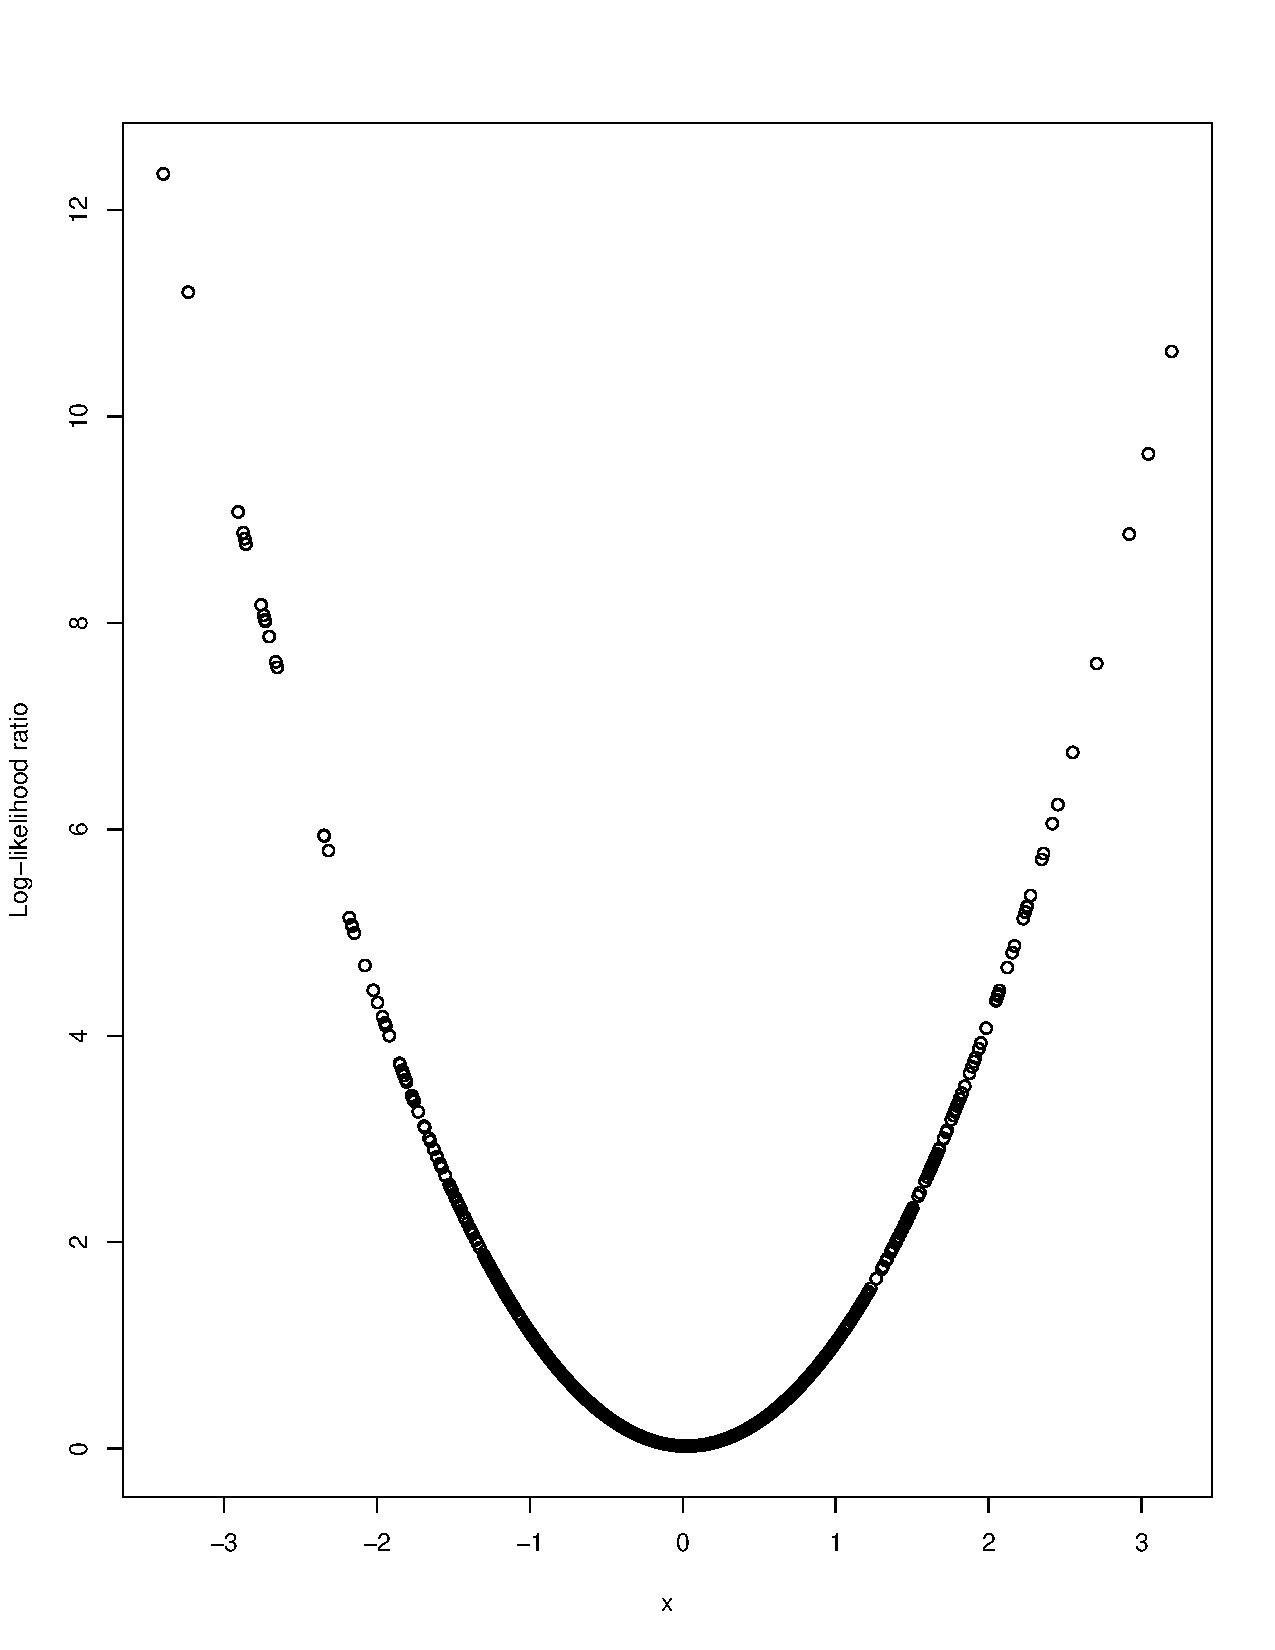
\includegraphics[scale = 0.6]{figures/loglik_ratio1.pdf}
    \caption{Log-likelihood ratio for $\theta = \left(0.05, 1\right)$, $\theta' = \left(0, 0.95\right)$  with $x \sim \mathcal{N}\left(0,1\right)$}
    \label{fig:loglik_ratio_gaussian}
\end{figure}
For a logistic regression model with parameters $\beta_0$ and $\beta_1$, the likelihood function for a single data point $y_i$ is given by 
\begin{equation}\label{eq:logist_likelihood}
\begin{split}
    L\left(\beta_0, \beta_1\right) &= p\left(x_i\right)^{y_i} \left(1 - p\left(x_i\right)\right)^{1-y_i} \\
    &= \left(\frac{1}{1 +  e^{-\beta0 -\beta_1 x_i}}\right)^{y_i} \left(1 +  \frac{1}{1 +  e^{-\beta0 -\beta_1 x_i}}\right)^{1 - y_i}. 
\end{split}
\end{equation}
Thus we have log-likelihood 
\begin{equation}\label{eq:logist_loglik_example}
\begin{split}
   \ell\left(\beta_0, \beta_1\right) &=  y_i\log\left(\frac{1}{1+e^{-\beta_0 - \beta_1x_i}}\right) + \left(1 -y_i\right) \log \left(1 - \frac{1}{1 + e^{-\beta_0 - \beta_1x_i}}\right)\\
    &= y_i\log\left(\frac{1}{1+e^{-\beta_0 - \beta_1 x_i}}\right) + \log\left(1 - \frac{1}{1 + e^{-\beta_0 - \beta_1x_i}}\right) - y_i\log\left(1 - \frac{1}{1 + e ^{-\beta_0 - \beta_1 x_i}}\right) \\
    & = y_i \log\left(\frac{\frac{1}{1+e^{-\beta_0 - \beta_1x_i}}}{-\left(1 - \frac{1}{1+e^{-\beta_0 - \beta_1 x_i}}\right)}\right) + \log \left(1 - \frac{1}{1 + e^{-\beta_0  -\beta_1 x_i}}\right)
    \\& = y_i\log\left(e^{\beta_0  +\beta_1 x_i }\right) + \log \left(1 - \frac{1}{1 + e^{-\beta_0 - \beta_1 x_i}}\right) \\
    & = y_i\left(\beta_0  +\beta_1 x_i\right) + \log \left(1 - \frac{1}{1 + e^{-\beta_0 - \beta_1 x_i}}\right) \\ 
    &= y_i\left(\beta_0 + \beta_1 x_i \right) + \log \left(\frac{1}{1 + e^{\beta_0 + \beta_1 x_i}}\right) = y_i\left(\beta_0 + \beta_1 x_i \right) - \log \left( 1 + e^{\beta_0  + \beta_1 x_i }\right)
    \end{split}
\end{equation}{}
Thus the log-likelihood ratio is given by 
\begin{equation}
\begin{split}
    \log\frac{L\left(\beta'\right)}{L\left(\beta\right)} &= \ell\left(\beta_0', \beta_1'\right) -  \ell \left(\beta_0,\beta_1\right)\\
    & = y_i\left(\beta_0' - \beta_0 + x_i \left(\beta_1' - \beta_1\right)\right) - \log \left(1 + e^{\beta_0' + \beta_1' \x_i}\right) + \log \left(1 + e^{\beta_0 +  \beta_1 x_i}\right) \\
    & = y_i\left(\beta_0' - \beta_0 + x_i\left(\beta_1' - \beta_1\right)\right) + \log \left(\frac{1 + e^{\beta_0 + \beta_1 x_i}}{1 + e^{\beta_0' + \beta_1' x_i}}\right) 
    \\
    & = \begin{cases}{} 
        \log \left(\frac{1 + e^{\beta_0 + \beta_1 x_i}}{1 + \beta_0' + \beta_1' x_i}\right) & if \quad y_i = 0 \\
        \beta_0' - \beta_0 + x_i \left(\beta_1' - \beta_1\right) + \log \left(\frac{1 + e^{\beta_0 + \beta_1 x_i}}{1 + e^{\beta_0' + \beta_1'x_i}}\right)  & if \quad y_i = 1
    \end{cases}
\end{split}
\end{equation}
The logistic regression log-likelihood is concave. 


We differentiate the log of the likelihood ratio with respect to $x_i$ to find the minimum of the log of the likelihood ratio. 
\begin{equation}
\begin{split}
    \frac{d}{dx} \left(\ell \left(\beta_0', \beta_1'\right) - \ell\left(\beta_0, \beta_1\right)\right) &= \begin{cases}
    \frac{d}{dx}\left(\log \left(\frac{1 + e^{\beta_0 + \beta_1 x}}{1 + e^{\beta_0' + \beta_1'x}}\right)\right) & if \quad y = 0 \\
    \frac{d}{dx} \left(\beta_0' -  \beta_0 + x \left(\beta_1' - \beta_1\right) + \log \left(\frac{1 + e^{\beta_0 + \beta_1 x}}{1 + e^{\beta_0' + \beta_1'}}\right)\right) & if \quad y = 1 \end{cases}
    \\ & = \begin{cases}
    \left(e^{\beta_0' + \beta_1'x} + 1\right)\frac{\left(\frac{\beta_1 e^{\beta_0 + \beta_1x}}{e^{\beta_0' + \beta_1'x + 1}} - \frac{d \left(e^{\beta_0 + \beta_1x} + 1\right)e^{\beta_0' + \beta_1'x}}{\left(e^{\beta_0' + \beta_1'x}+1\right)^2}\right)}{e^{\beta_0 + \beta_1x} + 1}
    \\\left(e^{\beta_0' + \beta_1'x} + 1\right)\frac{\left(\frac{\beta_1 e^{\beta_0 + \beta_1x}}{e^{\beta_0' + \beta_1'x + 1}} - \frac{d \left(e^{\beta_0 + \beta_1x} + 1\right)e^{\beta_0' + \beta_1'x}}{\left(e^{\beta_0' + \beta_1'x}+1\right)^2}\right)}{e^{\beta_0 + \beta_1x} + 1} + \beta_1' - \beta_1
    \end{cases}
\end{split}
\end{equation}
\todo{Se i artikkel, L-Lipschitz osv. }
\todo{vanskelig å løse for $x$.}
\begin{figure}
    \centering
    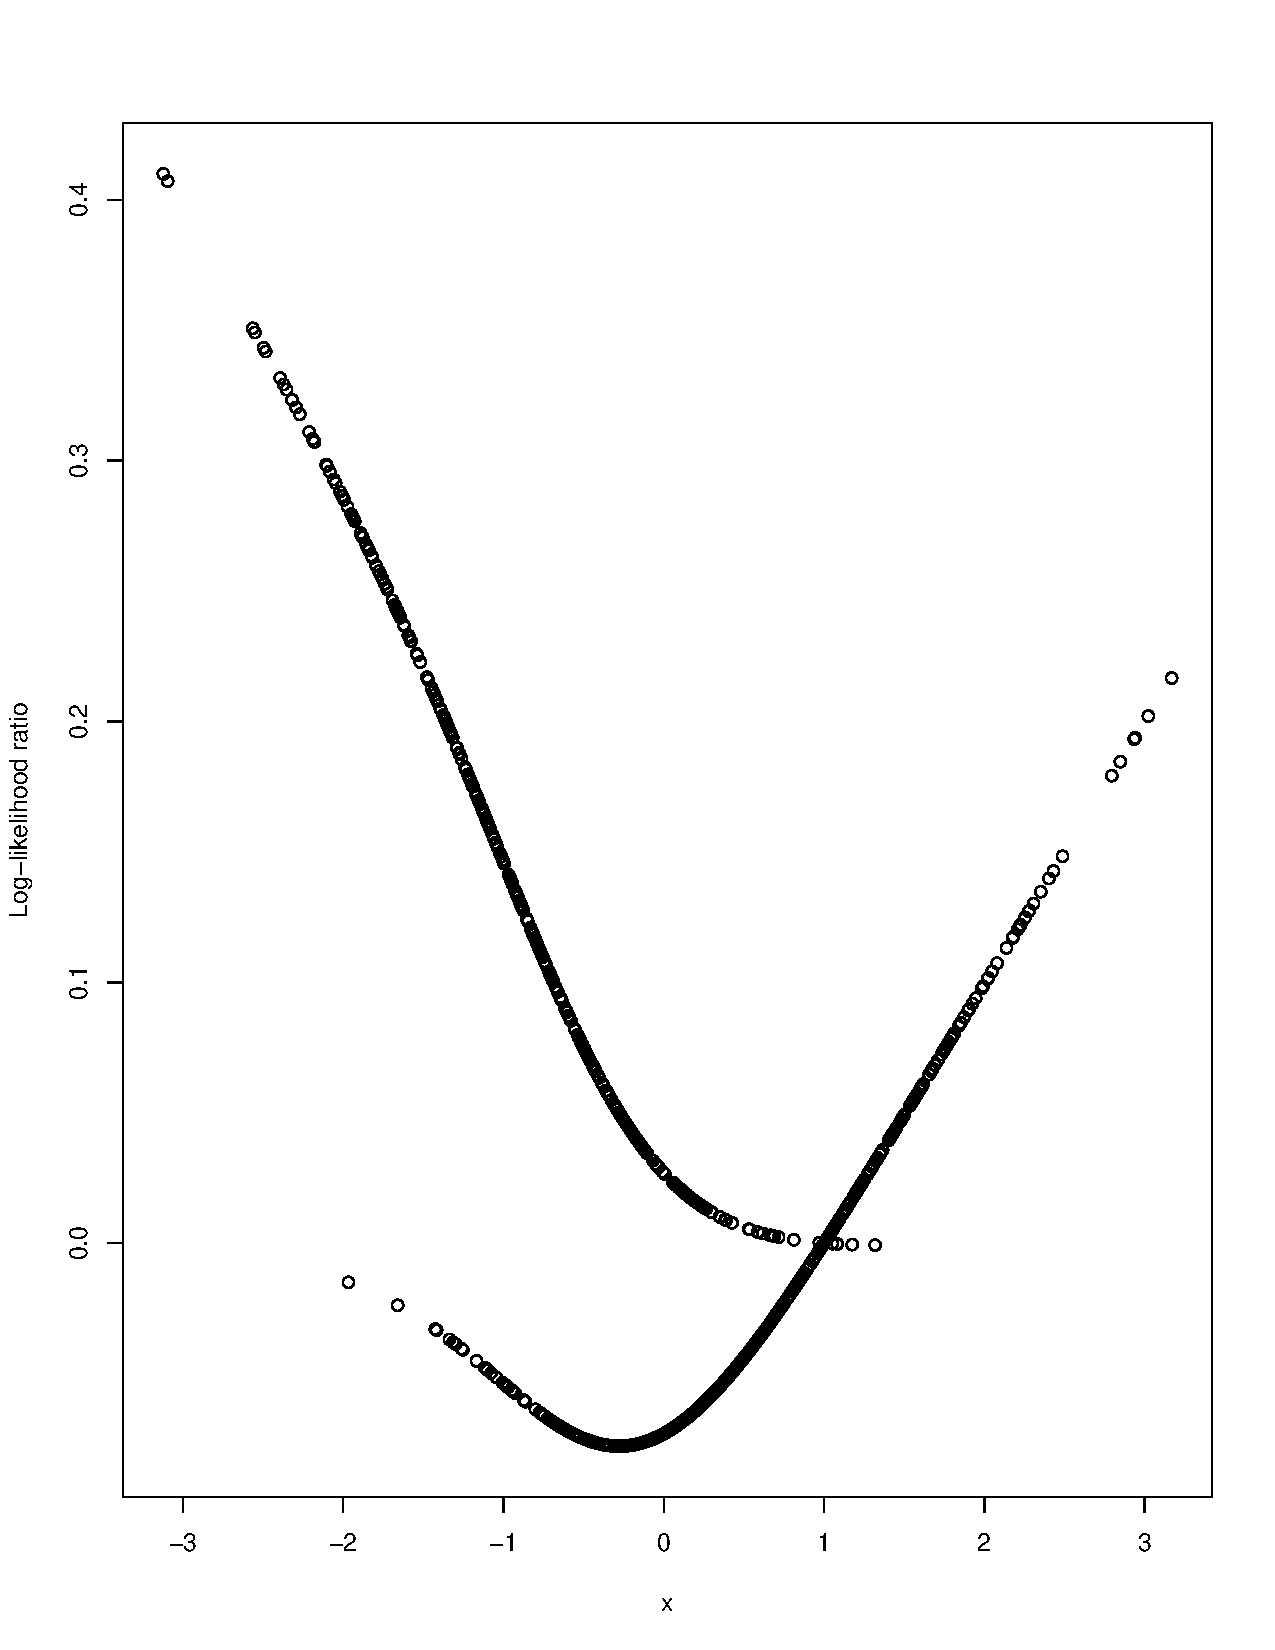
\includegraphics[scale = 0.7]{figures/loglik_ratio_logistic.pdf}
    \caption{Log-likelihood ratio for $\theta = \left(\beta_0, \beta_1\right) = \left(0.95, 2.05\right), \theta' = \left(1.05, 1.95\right)$, $\theta_{True} = \left(1, 2\right)$}
    \label{fig:loglik_ratio_logistic}
\end{figure}{}
\begin{figure}
    \centering
    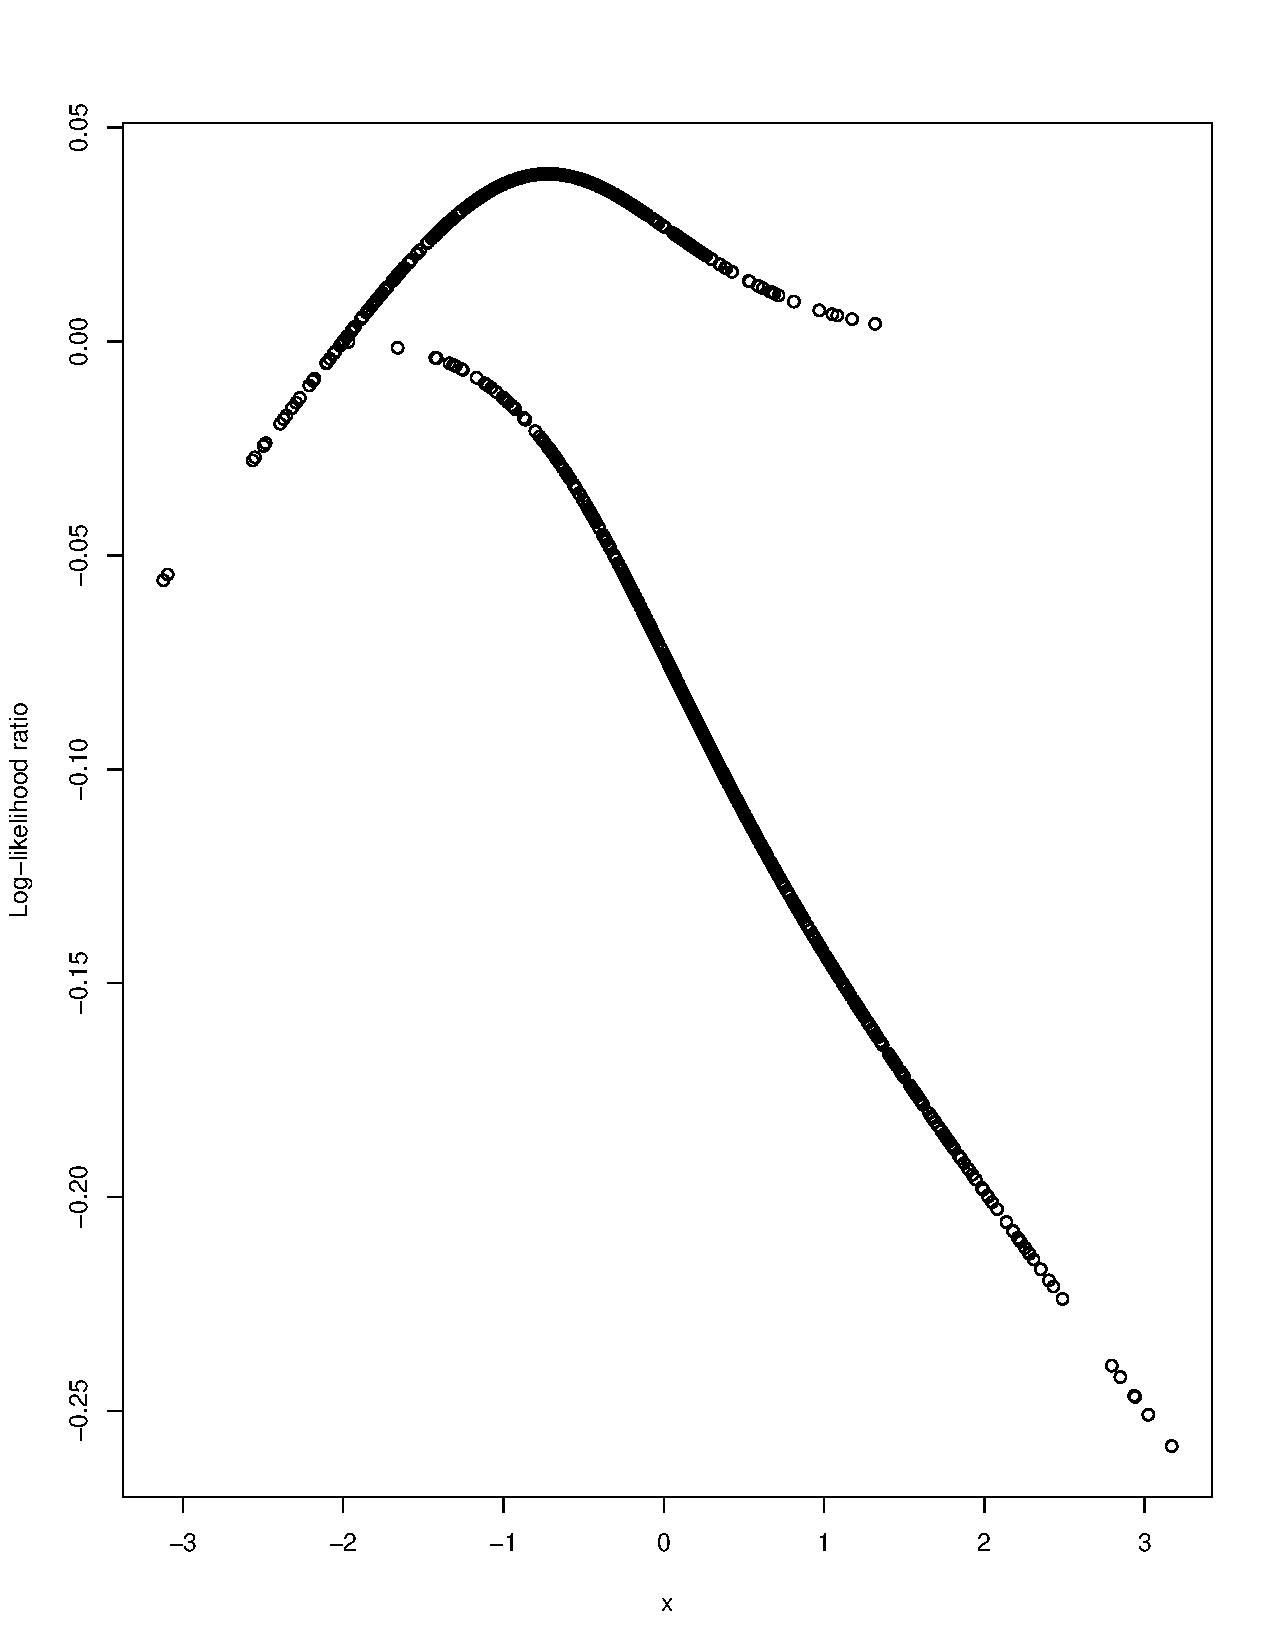
\includegraphics[scale = 0.7]{figures/loglik_ratio_logist2.pdf}
    \caption{Log-likelihood ratio for $\theta = \left(\beta_0, \beta_1\right) = \left(0.95, 2.0\right), \theta' = \left(1.05, 2.2\right)$}
    \label{fig:my_label}
\end{figure}{
A function on the form $ax + b$ is both convex and concave \todo{referanse}, while $\log\left(1 + e^x\right)$ is convex \todo{proof}. 
Thus $\log\left(\frac{1 + e^{\beta_0 + \beta_1 x}}{1 + e^{\beta_0' + \beta_1'x}}\right) = \log\left(1 + e^{\beta_0 + \beta_1}\right) - \log\left(1+ e^{ \beta_0' + \beta_1'x}\right)$ is convex if 
\begin{equation*}
\begin{split}
    \log\left(1 + e^{\beta_0 + \beta_1x}\right) &> \log\left(1 + e^{\beta_0' + \beta_1' x}\right)  \\
    \implies 1 + e^{\beta_0 + \beta_1x} &> 1 + e^{\beta_0' + \beta_1'x} \\
    \implies \beta_0 + \beta_1 x &> \beta_0' + \beta_1'x.
\end{split}{}
\end{equation*}
Similarly, the log-likelihood ratio is concave if 
\begin{equation*}
    \beta_0 + \beta_1 x < \beta_0' + \beta_1'x. 
\end{equation*}
The maximum absolute value of the log-likelihood ratio will thus be either at the extreme $x$-values or at the $x$-value closest to the global maximum or minimum for concave and convex log-likelihood ratios respectively.  To find the global maximum or minimum of the log-likelihood ratio, we have to differentiate and set equal to zero, solve for $x$, and find the $x$-value closest to the $x$-value of the global maximum/minimum. \todo{how is this in the case of multidimensional $x$?}
\section{Linear regression}
In the case of simple linear regression, i.e. $y_i \sim \mathcal{N}\left(\beta_0 + \beta_1 x_i, \sigma^2\right)$, we cannot find such a simple rule as in the case of normally distributed data dependent only on the parameters. 
For simple linear regression, the log-likelihood ratio is given by 
\begin{equation}
\begin{split}
    \log \frac{L\left(\theta'\right)}{L\left(\theta\right)} &= \log \frac{L\left(\beta_0', \beta_1', \sigma'\right)}{L\left(\beta_0, \beta_1, \sigma\right)}  \\
    & = \ell\left(\beta_0, \beta_1, \sigma\right) - \ell\left(\beta_0, \beta_1, \sigma\right) \\
    & = -\log\sigma' + \log\sigma - \frac{\left(y - \beta_0' - \beta_1'x\right)^2}{2\sigma'^2} + \frac{\left(y - \beta_0 - \beta_1x\right)^2}{2\sigma^2} \\
    & = \log \sigma - \log \sigma' - \frac{y^2 - 2y\beta_0'  - 2y\beta_1' + \beta_0'^2 + 2\beta_0'\beta_1'x + \beta_1'^2x^2 }{2\sigma'^2} \\ &+ \frac{y^2 - 2y\beta_0 - 2y\beta_1x + \beta_0^2 + 2\beta_0\beta_1x + \beta_1^2x^2}{2\sigma^2}
    \end{split}
\end{equation}
We plot this log-likelihood ratio as a function of $y$ to see how it behaves. 
\begin{figure}[H]
    \centering
    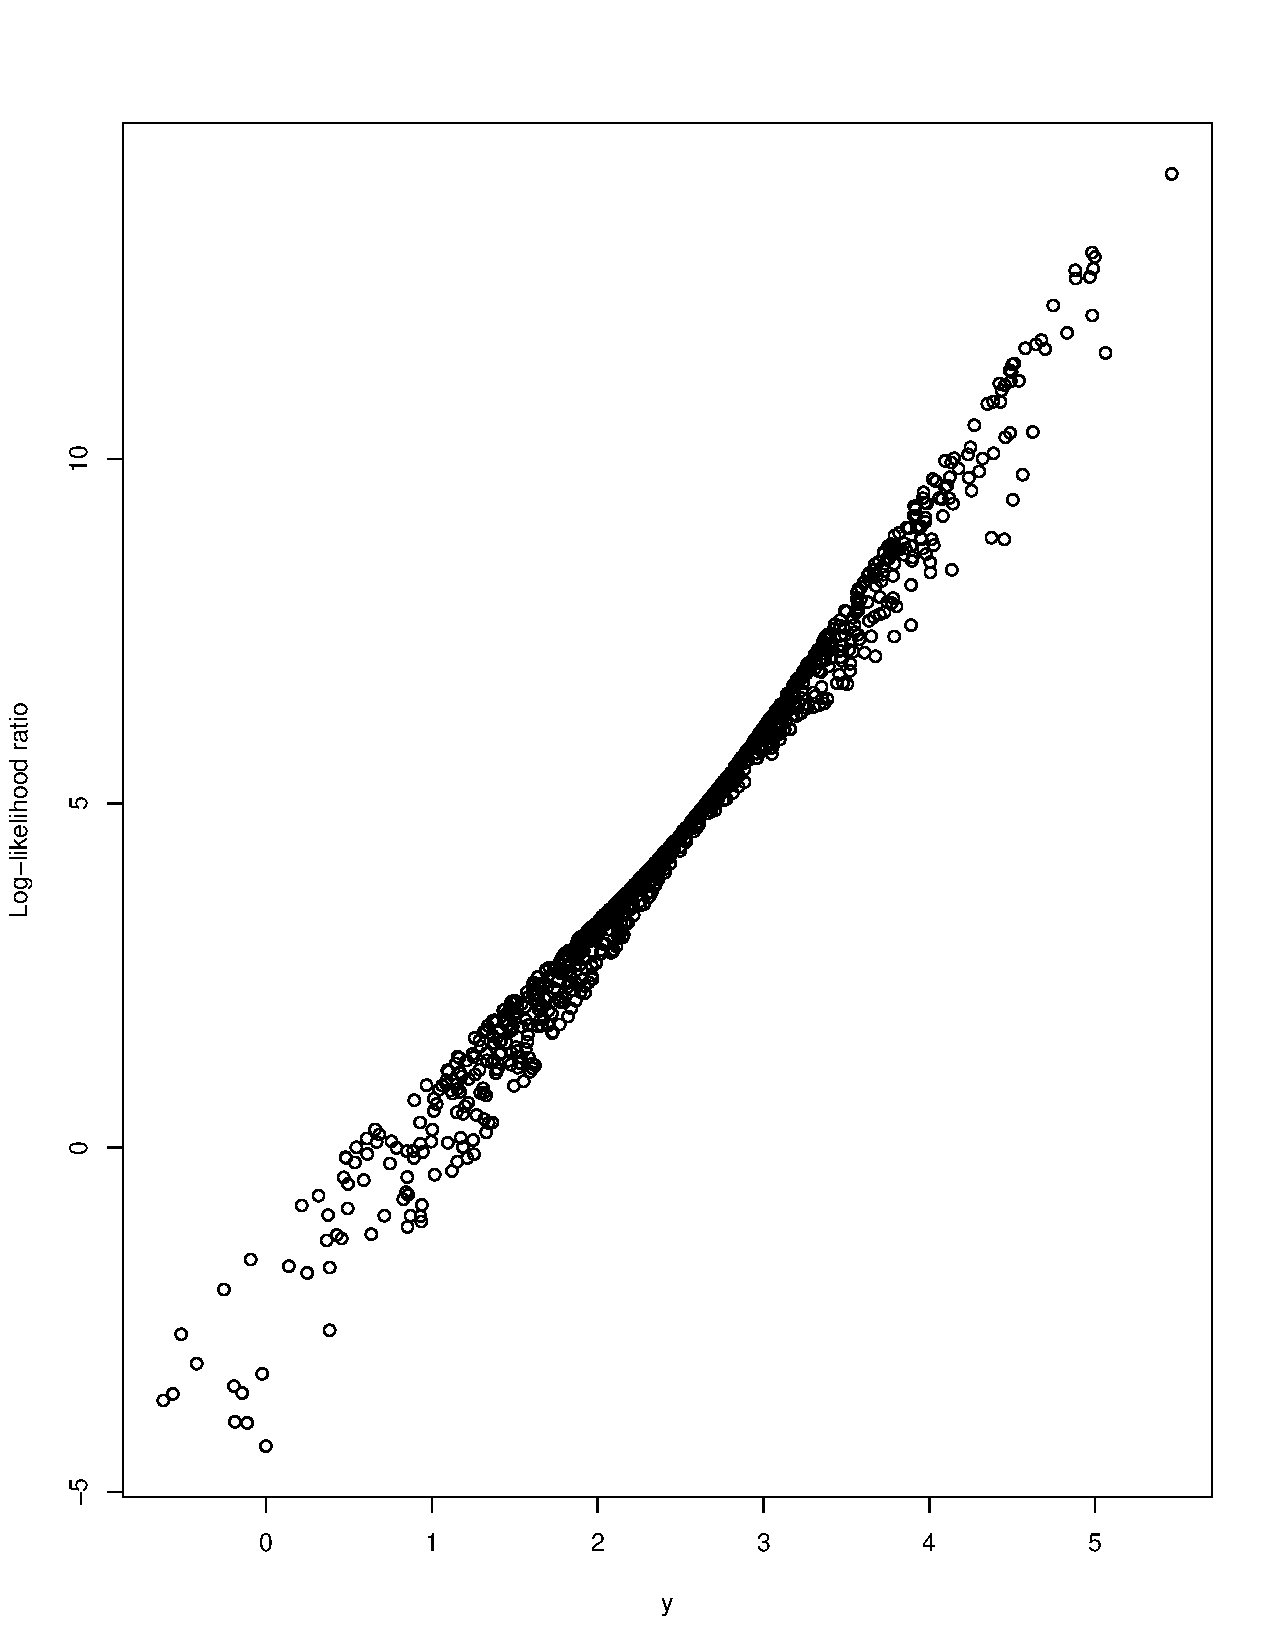
\includegraphics[scale = 0.7]{figures/loglik_ratio2.pdf}
    \caption{Caption}
    \label{fig:my_label}
\end{figure}{}
\todo{Paragraph about calculation of $c$, and how to do it in a smarter way}
Then, the difference between the estimate and the true value can be controlled, and it is this knowledge of the precision of the estimate that is utilized to limit the required computational power.
Since $\theta'$ is to be accepted if $\Lambda_N\left(\theta, \theta'\right) > \psi\left(u, \theta, \theta'\right)$,  $\theta'$ will be correctly accepted with at least probability $1 - \delta_t$ if  the following holds 
\begin{equation}\label{eq:conf_sampler_condition}   \mid\Lambda_t^{\star}\left(\theta, \theta'\right) - \psi\left(u, \theta, \theta'\right)\mid \:>\: c_t
\end{equation}
What they do is start with a small sub sample, i.e. $t \ll n$, and if \eqref{eq:conf_sampler_condition} holds, $\theta'$ is accepted. 
Otherwise, the size of the sub sample is increased, and it is again tested if \eqref{eq:conf_sampler_condition} holds.
This procedure is repeated until either the condition of \eqref{eq:conf_sampler_condition} holds, or the sub sample contains all the data points and \eqref{eq:conf_sampler_condition} does not hold, according to \textbf{step 21}. \todo{reference line in algorithm}
Next, to decide whether or not to accept the proposal $\theta'$, 
they check whether $\Lambda^{\star} > \psi \left(u, \theta, \theta ' \right)$. 
The proposal is accepted if $\Lambda^{\star} >  \psi \left(u, \theta, \theta ' \right)$ and rejected otherwise.   
The stopping time $T$ denotes the number of data points considered before stopping, i.e. 
\begin{equation}\label{eq:T_stopping}
    T = \min\left(N, \inf\left\{t\geq 1 :\; \mid \Lambda_t^{\star}\left(\theta, \theta'\right) - \psi\left(u, \theta, \theta'\right)\mid \;\leq c_t\right\}\right)
\end{equation}
\todo{finn riktige symboler}
They let $\epsilon$ be the event

\begin{equation}\label{eq:epsilon}
    \mathbb{\epsilon} = \cap_{t\geq 1}\left\{\mid\Lambda_N\left(\theta, \theta'\right) - \Lambda_T^{\star} \left(\theta, \theta'\right) \mid \leq c_t\right\}.   
\end{equation}
They apply De Morgan's law 
\begin{equation}
    \left(\cap_{i=1}^n A_i\right)^c = \cup_{i=1}^n A_i^c
\end{equation}
So, 
\begin{equation}
\begin{split}
     \epsilon^c = \left(\cap _{t\geq 1}\left\{\mid \Lambda_N\left(\theta, \theta'\right) - \Lambda_T^{\star}\left(\theta, \theta'\right) \mid \leq c_t\right\}\right)^c &= \cup_{t\geq 1} \left\{\mid \Lambda_N\left(\theta, \theta'\right) - \Lambda_t^{\star}\left(\theta, \theta'\right) \mid \leq c_t\right\}^c \\
\end{split}
\end{equation}
and 
\begin{equation}
\begin{split}
    \epsilon &= \left(\epsilon^c\right)^c = \left(\cup_{t\geq 1} \left\{\mid \Lambda_N\left(\theta, \theta'\right) - \Lambda_t^{\star}\left(\theta, \theta'\right) \mid \leq c_t \right\}^c\right)^c 
\end{split}
\end{equation}{}
Then, by Boole's inequality
\begin{equation}\label{eq:Boole}
    P\left(\cup_i A_i \right) \leq \sum_{i} P\left(A_i\right)
\end{equation}
\begin{equation}
\begin{split}
       P\left(\epsilon^c\right) &= P\left(\cup_{t\geq 1} \left\{\mid\Lambda_N\left(\theta, \theta'\right)- \Lambda_t^{\star}\left(\theta, \theta'\right) \mid \leq c_t\right\}^c\right) \\
    1 - P\left(\epsilon\right) &\leq \sum_{t\geq 1} P\left(\left(\mid \Lambda_N\left(\theta, \theta'\right) - \Lambda_t^{\star}\left(\theta, \theta'\right) \mid \leq c_t \right)^c\right) \\ 
    1 - P\left(\epsilon\right) &\leq \sum_{t\geq 1} 1 - \left(1 - \delta_t\right) \\
    P\left(\epsilon\right) &\geq 1 - \sum_{t\geq 1} \delta_t \geq 1 - \delta.  
\end{split}
\end{equation}
As the correct decision is always taken at the event $\epsilon$, and since $P\left(\epsilon\right)\geq 1- \delta$, the correct decision will be taken with probability of at least $1 - \delta$. 
 \subsubsection{Convergence to correct stationary distribution}
 As we saw in \ref{subsec:mh}, the transition kernel of the Metropolis-Hastings algorithm,
 $P(\theta, \theta')$, is given by
 \begin{equation*}
     P\left(\theta, d\theta'\right) = \alpha\left(\theta'\right)g\left(\theta'\mid\theta\right)d\theta' + \delta_{\theta}\left(d\theta'\right)\left(1 - \int\alpha\left(\theta, \vartheta\right)g\left(\vartheta\mid\theta\right) d\vartheta\right). 
 \end{equation*}
\begin{equation*}
\begin{split}
     \alpha\left(\theta, \theta'\right) &= \min\left(1,\; \frac{\pi\left(\theta'\right)}{\pi\left(\theta\right)}\frac{q\left(\theta\mid\theta'\right)}{q\left(\theta'\mid\theta\right)} \right) \\
     & = E \;\mathbb{1} \left(\Lambda_N\left(\theta, \theta'\right)> \psi \left(u, \theta, \theta' \right)\right)
\end{split}     
\end{equation*}
is the regular MH acceptance probability. The acceptance probability for the adaptive subsampler is given by 
\begin{equation}\label{eq:approx_accept}
    \Tilde{\alpha} = E \; \mathbb{1} \left(\Lambda_T^{\star}\left(\theta, \theta'\right) > \psi\left(u, \theta, \theta'\right)\right). 
\end{equation} 
\cite{Bardenet:2} propose the following lemma regarding the difference between $\alpha$ and $\Tilde{\alpha}$
\begin{lemma}\label{lemma:acceptance}
For any $\theta, \theta' \in \Theta$ we have $\mid \alpha - \Tilde{\alpha} \mid \leq \delta$
\end{lemma}
where $\delta$ is the user specified $\delta$ from \eqref{eq:concentration}. To prove Lemma \ref{lemma:acceptance}, we follow the supplementary material of \cite{Bardenet:2}. 
\begin{proof} From the definition of $\alpha$ and $\Tilde{\alpha}$, we have 
\begin{equation*}
\alpha - \Tilde{\alpha} = E\left[\; \mathbb{1}\left(\Lambda_N\left(\theta, \theta'\right) > \psi\left(u, \theta, \theta'\right)\right) - \mathbb{1}\left(\Lambda_T^{\star}\left(\theta, \theta'\right) > \psi\left(u, \theta, \theta'\right)\right)\right]    
\end{equation*}
which we can rewrite to
\begin{equation*}
    E\left[\; \mathbb{1}\left(\Lambda_N\left(\theta, \theta'\right) > \psi\left(u, \theta, \theta'\right)\right) - \mathbb{1}\left(\Lambda_T^{\star}\left(\theta,\theta'\right) > \psi\left(u, \theta, \theta'\right)\right)\mid T < N \right] 
\end{equation*}
since for $T = n$, $\Lambda_T^{\star}\left(\theta, \theta'\right) = \Lambda_N\left(\theta, \theta'\right)$, so  $\alpha = \Tilde{\alpha}$. We want to bound the absolute difference between $\alpha$ and $\Tilde{\alpha}$, $\mid \alpha - \Tilde{\alpha}\mid$. So we apply Jensen's inequality: 
\begin{equation}\label{eq:jensen}
\phi\left(E\left[X\right] \right) \leq E\left[\phi\left(X\right)\right] 
\end{equation}
for some convex function $\phi$. Since the absolute value, $\mid \cdot\mid$, is a convex function, we have  
\begin{equation*}
\begin{split}
\mid \alpha - \Tilde{\alpha}\mid &= 
    \mid E\left[\mathbb{1}\left(\Lambda_N\left(\theta, \theta'\right) > \psi \left(u, \theta, \theta'\right)\right) - \mathbb{1}\left(\Lambda_T^{\star}\left(\theta, \theta'\right) > \psi\left(u, \theta, \theta'\right)\right)\mid T < N\right]\mid 
    \end{split}
\end{equation*}
\begin{equation*}
    \leq E\left[\mid \mathbb{1}\left(\Lambda_N\left(\theta, \theta'\right) > \psi\left(u, \theta, \theta'\right)\right) - \mathbb{1}\left(\theta, \theta'\right) > \psi\left(u, \theta, \theta'\right)\mid T<  N\right]
\end{equation*}
If we have $\mid \mathbb{1}\left(\Lambda_N\left(\theta, \theta'\right) > \psi\left(u, \theta, \theta'\right)\right) - \mathbb{1}\left(\Lambda_T^{\star}\left(\theta, \theta'\right) > \psi\left(u, \theta, \theta'\right)\right)\mid = 1$ (\textbf{at some iteration of the Markov chain}) and using the definition of $T$ given in \eqref{eq:T_stopping} \textbf{we} see that $\mid \Lambda_n\left(\theta, \theta'\right) - \Lambda_T^{\star}\left(\theta, \theta'\right) \mid \geq c_T$, so
\begin{equation*}
\begin{split}
\mid \alpha - \Tilde{\alpha}\mid &\leq
     E\left[\mid\mathbb{1}\left(\Lambda_N\left(\theta, \theta'\right)> \psi\left(u, \theta, \theta'\right)\right) -\mathbb{1}\left( \Lambda_T^{\star}\left(\theta, \theta'\right)>\psi\left(u, \theta, \theta'\right)\right)\mid T<N \right] \\ &= E\left[\mid \mathbb{1}\left(\mid \Lambda_N\left(\theta, \theta'\right) - \Lambda_T^{\star}\left(\theta, \theta'\right)\mid \geq c_T\right)\mid T<N\right]\\ &= P\left(\mid\Lambda_N\left(\theta, \theta'\right) - \Lambda_T^{\star}\left(\theta, \theta'\right)\mid \geq c_T \mid T < N \right) \\
     & \leq P\left(\cup_{t \geq 1} \mid \Lambda_N\left(\theta, \theta'\right) - \Lambda_t^{\star}\mid \geq c_t \right) = P\left(\epsilon^c\right) = 1 - \left( 1 - \delta\right) = \delta 
\end{split}
\end{equation*}

\textbf{where the last inequality is valid since $T$ is the last of the $t$'s (by definition of $T$)}
\end{proof}
They use Lemma \ref{lemma:acceptance} to prove that the invariant distribution of the Markov chain using the adaptive subsampler is a controlled estimate of the true target distribution. 
\begin{proposition}\label{prop:dist}
Assume that $P$ is uniformly geometrically ergodic, i.e. there exists an integer $n$ and a probability measure $\nu$ on $\left(\Theta, \mathcal{B}\left(\Theta\right)\right)$ such that, for all $\theta \in \Theta$, $P^m\left(\theta, \cdot\right) \geq \left(1 - \rho\right)\nu\left(\cdot\right)$. Hence there exists $A < \infty$ such that
\begin{equation*}
    \forall \theta \in \Theta \forall k > 0, \quad \lVert P^k\left(\theta, \cdot\right) - \pi \rVert_{TV} \leq A\rho^{\lfloor k/m \rfloor} 
\end{equation*}
Then there exists $B < \infty$ and a probability distribution $\Tilde{\pi}$ such that 
\begin{equation*}
    \forall \theta \in \Theta, \forall k > 0, \quad \lVert \Tilde{P}^k\left(\theta, \cdot\right) - \Tilde{\pi}\rVert_{TV} \leq B\left[ 1 - \left(1- \delta\right)^m \left(1-\rho\right)\right]^{\lfloor k/m\rfloor}
\end{equation*}
and $\Tilde{\pi}$ satisfies 
\begin{equation*}
    \lVert \Tilde{\pi} - \pi \rVert \mid_{TV} \leq \frac{A m\delta}{1-\rho} 
\end{equation*}
\end{proposition}
For the proof of \ref{prop:dist}, we follow the supplementary material of \cite{Bardenet:2}. 
With transition kernel for the Metropolis-Hastings algorithm given by 
\todo{Skal denne være et annet sted?}
\begin{equation*}
    P\left(\theta, d\theta'\right) = \alpha\left(\theta, \theta'\right)g\left(\theta'\mid \theta\right)d\theta' + \delta_{\theta}\left(d\theta\right)\left(1 - \int(\alpha\left(\theta, \vartheta\right)g\left(\vartheta\mid\theta\right) d\vartheta  \right) 
\end{equation*}
\begin{proof}
The transition kernel for the \textbf{approximate acceptance probability} is given by 
\begin{equation*}
    \Tilde{P}\left(\theta, d\theta'\right) = \Tilde{\alpha}\left(\theta, \theta'\right)g\left(\theta'\mid \theta \right) d\theta' + \delta_{\theta}\left(d\theta'\right)\left(1 - \int\Tilde{\alpha}\left(\theta, \vartheta\right)g\left(\vartheta\mid \theta\right) d\vartheta \right) 
\end{equation*}
If we insert \eqref{eq:approx_accept}, we get 
\begin{equation}
\begin{split}
    \Tilde{P}\left(\theta, d\theta'\right) &=  E\mathbb{1} \left(\Lambda_T^{\star}\left(\theta, \theta'\right) > \psi\left(u, \theta, \theta'\right)\right)g\left(\theta \mid \theta' \right) d\theta'\\
    &+ \delta_{\theta} \left(d\theta'\right)\left(1 - \int E \mathbb{1}\left(\Lambda_T^{\star}\left(\theta, \vartheta\right) > \psi \left(u,  \theta, \vartheta\right) \right)g\left(\vartheta \mid \theta\right) d\vartheta  \right)
\end{split}
\end{equation}
\end{proof}
\todo{fullfør}
\section{Adaptive subsampler using proxies as control variates}\label{sec:adap_subsampl}
Bardenet et al. \cite{Bardenet:1} propose using a confidence sampler with proxies for the likelihood, which act as control variates. 
Control variates are used to reduce the variance of an estimator by relating the original estimator to a known quantity. 
Say we want to estimate $EX = \theta$ with the unbiased estimator $\hat{\theta}$. Suppose we also have another random variable (\textbf{output variable}) $Y$ where the expectation of $Y$, $EY = \mu$ is know. 
We define $$\hat{\theta}_{CV} = \hat{\theta} + c\left(Y - \mu\right) $$  Then, $\hat{\theta}_{CV}$ will also be  an unbiased estimator of $\theta$, and if we choose $c$, correctly, it will also have a smaller variance than $\hat{\theta}$. 
This we can easily show by \begin{equation*}
\begin{split}
    \mathrm{Var}\;\hat{\theta}_{CV}  &= \mathrm{Var}\left[\hat{\theta} + c\left(Y - \mu\right)\right]
     = \mathrm{Var}\left(\hat{\theta} - cY\right) \\ & = \mathrm{Var}\;\hat{\theta} + c^2\mathrm{Var}\;Y + 2c\mathrm{Cov}\left(\hat{\theta}, Y\right)
\end{split}
\end{equation*}
We want to find the $c$ that minimizes the variance of $\hat{\theta}_{CV}$. 
\begin{equation}\label{eq:control_var}
\begin{split}
    \frac{\partial}{\partial c} \mathrm{Var}\; \hat{\theta}_{CV} &= 2c\mathrm{Var}\;Y + 2\mathrm{Cov}\left(\hat{\theta}, Y\right) = 0 \\
    & \implies c = - \frac{\mathrm{Cov}\left(\hat{\theta}, Y\right)}{\mathrm{Var}\;Y}
\end{split}
\end{equation}
We calculate the second derivative to show that the result from (\ref{eq:control_var}) is indeed a minimum
\begin{equation*}
    \frac{\partial^2}{\partial c^2} \mathrm{Var}\; \hat{\theta}_{CV}  = 2\mathrm{Var}\; Y > 0 
\end{equation*}
so $c = -\frac{\mathrm{Cov}\left(\hat{\theta}, Y\right)}{\mathrm{Var}\;Y}$ reduces the variance to a minimum. \\
The confidence sampler introduced in \cite{Bardenet:1} is an alteration of the confidence sampler in \cite{Bardenet:2}. 
The bottleneck of the confidence sampler introduced in \cite{Bardenet:2} is the calculation of the expectation with respect to $\pi\left(\theta\right)q\left(\theta \mid \theta'\right)$ of the variance of the log likelihood ratio $\log \left(p\left(x\mid \theta\right)\right) / \log \left(p\left(x\mid \theta\right)\right)$ with respect to the empirical distribution of the observations.
In order to lower the variance, Bardenet et al. are inspired by Maclaurin and Adams and introduce a proxy, $\powerset$, which is a function of $\theta$ and $\theta'$ and defined for each data point $i$, and let the following be restrictions on $\powerset_i\left(\theta, \theta'\right)$ for any $\theta, \theta' \in \Theta$. 
\begin{enumerate}
    \item $\powerset_i\left(\theta, \theta'\right) \approx \ell_i\left(\theta'\right) - \ell_i\left(\theta\right)$
    \item $ \sum_{i = 1}^n \powerset_i\left(\theta, \theta'\right)$ can be computed cheaply
    \item $\left| \ell_i\left(\theta'\right) - \ell_i\left(\theta\right) - \powerset_i\left(\theta, \theta'\right)\right|$ can be bounded uniformly in $1\leq i \leq n$ and the bound is cheap to compute. 
\end{enumerate}
Bardenet et al. rewrite Algorithm \ref{algo:MH} using 
The idea of Bardenet et al. \cite{Bardenet:2} is to use a Monte Carlo estimate of $\Lambda_N$ using only a subsample of data,  and then do MCMC similarly to Algorithm \ref{algo:MH_rewritten}. 
\begin{equation*}
    \Lambda^{\star}_t\left(\theta, \theta'\right) = \frac{1}{t}\sum_{i = 1}^t \log\left[\frac{p\left(x_i\mid\theta'\right)}{p\left(x_i\mid \theta\right)}\right] 
\end{equation*}
Where $x^{\star}_1, \ldots, x^{\star}_t$ are drawn uniformly from $\{x_1, \ldots, x_n\}$ without replacement.  
They quantify the precision of the estimate $\Lambda_t^{\star}$ by using concentration inequalities, like Hoeffding's inequalty.  \begin{equation}\label{eq:Hoeffdings}
    P\left(\Lambda_N \left(\theta, \theta'\right) - \Lambda_t^{\star}\left(\theta, \theta'\right) \geq c_t \right) \leq \delta_t \iff P\left(\Lambda_N\left(\theta, \theta'\right) - \Lambda_t^{\star}\left(\theta, \theta'\right) \leq c_t\right) \geq 1 - \delta_t 
\end{equation}
Using (\ref{eq:Hoeffdings}), they can control the maximum probability of making a wrong decision by construction of $c_t$.  \textbf{figure more out of this}. \textbf{How to reference to line in algo?}. 
\textbf{How is this related to confidence samplers?} \textbf{proxy acts as a controlvariate in the concentration inequation?}
\begin{algorithm}[H]
    \caption{Confidence Sampler}
    \label{algo:conf_sampl}
    \begin{algorithmic}[1] % The number tells where the line numbering should start
    \Function{ConfidenceSampler}{$p\left(x\mid \theta \right), p\left(\theta\right), q\left(\theta'\mid \theta\right), \theta_0, N_{iter}, \chi, \left(\delta_t\right), C_{\theta, \theta'}$}
       \For {$i \gets 1 \ldots N_{iter}$}
       \State $\theta = \theta^{\left(i-1\right)}$
       \State $\theta' \sim q\left(\cdot|\theta\right)$
       \State $u \sim \mathcal{U}\left(0,1\right)$
       \State$\psi\left(u, \theta, \theta'\right) = \frac{1}{n}\log\left[u\frac{p\left(\theta\right)q\left(\theta'\mid \theta\right)}{p\left(\theta'\right)q\left(\theta \mid\theta'\right)}\right]$
       \State $t = 0$
       \State $t_{look} = 0$
       \State $\Lambda^{\star} = 0$
       \State $\chi^{\star} = \emptyset$
       \State $b = 1$
       \State $\textsc{DONE} = \textsc{FALSE}$
       \While{$\textsc{DONE} = \textsc{FALSE}}$
       \State $x_{t+1}^{\star}, \ldots, x_b^{\star} \sim_{w.o\;repl.} \chi \setminus \chi^{\star}$
       \State $\chi^{\star} = \chi^{\star} \bigcup \left\{x_{t+1}^{\star}, \ldots, x_b^{\star}\right\}$
       \State $\Lambda^{\star} = \frac{1}{b} \left(t\Lambda^{\star} + \sum_{n = t+1}^b \log \left[\frac{p\left(x_n^{\star}\mid\theta'\right)}{p\left(x_n^{\star}\mid \theta\right)}\right]\right)$
       \State $t = b$
       \State $c = c_t\left(\delta_{t_{look}}\right)$
       \State $t_{look} = t_{look} + 1$
       \State $b = n\wedge \lceil \gamma t \rceil$
       \If{$|\Lambda^{\star} - \psi\left(u, \theta,\theta'\right) | \geq c \OR t = n$}\label{confidence:break_while}
       \State $\textsc{DONE} = \textsc{TRUE}$
       \EndIf
       \EndWhile
       \If{$\Lambda^{\star} > \psi\left(u, \theta, \theta'\right)$}
       \State{$\theta^{\left(i\right)} = \theta'$}
       \Else 
       \State{$\theta^{\left(i\right)} = \theta$}
       \EndIf
       \EndFor
       \State \Return $\left(\theta^{\left(i\right)}\right)_{i = 1, \ldots, N_{iter}}$
       \EndFunction
    \end{algorithmic}
\end{algorithm}
\todo{skriv mer}
\section{Quiroz et al. 2019}
\cite{quiroz2019speeding} suggest adding control variates to the naive subsampling method to control the variance of the log-likelihood ratio. They use a Taylor expansion about the parameter space in addition to a Taylor expansion about the nearest centroid in data space. The centroid in data space is calculateted using the clustering algorithm given below. 
\todo{Kan ikke kalle data for $z$}
\begin{algorithm}
\caption{Data clustering}
\label{algo:clustering}
\begin{algorithmic}[1]
    \Function{clustering}{$x, y, \epsilon$}
    \State $z_i \gets \left(y_i, x_i\right)^T$
    \State $z \gets \left(z_1^T, \ldots z_n^T\right)^T $
    \State $I \gets \left(0, \ldots, 0\right)^T$ 
    \State $\left(j,k\right) \gets \left(0,0\right)$
    \While{$\sum I_j \neq N$}
    \If{$I_j = 0$}
    \State $C_k \gets \left\{i; \lVert z_j - z_i \rVert \leq \epsilon\right\}  $
    \State $N_k = \left| C_k\right|$ 
    \State $z^{c_k} = \frac{1}{N_k} \sum_{i\in C_k} z_i$
    \State $I_{c_k} \gets 1$
    \State $k\gets k+1$
    \EndIf
    \State $j \gets j+1$
    \EndWhile
    \State $K\gets k$
    \State \textbf{return}$\left\{z^{c_k}\right\}_{k = 1}^K, \; \left\{C_k\right\}_{k=1}^K$
    \EndFunction
    \end{algorithmic}
\end{algorithm}{}
After clustering the data as described by Algorithm \ref{algo:clustering}, \cite{quiroz2019speeding} make a Taylor approximation of the log-likelihood $\ell_i\left(z_i;\theta\right)$ $q\left(z_i, \theta\right)$ about the centroid of the cluster that $z_i$ belongs to.  
\begin{equation}
    q_{i, n}\left(\theta\right) = q\left(z_i;\theta\right) = \ell\left(z^c, \theta\right) + \nabla_z \ell\left(z^c; \theta\right)^T \left(z_i - z^c \right) + \frac{1}{2}\left(z_i - z^c\right)^T H\left(z^c;\theta\right)\left(z_i - z^c\right)
\end{equation}
With $H\left(z^c; \theta\right)$ the Hessian evaluated at $z^c$. 
They define $d_{i, n} = \ell_i\left(\theta\right) - q_{i,n}\left(\theta\right)$ and 
\begin{equation*}
\begin{split}
    \mu_{d,n}\left(\theta\right) &\coloneqq \frac{1}{n}\sum_{i = 1}^n d_{i,n}\left(\theta\right) \\
    \sigma_{d,n} &\coloneqq \frac{\sum_{i=1}^n\left(d_{i,n}\left(\theta\right) - \mu_{d,n}\left(\theta\right)\right)^2}{n}
\end{split}
\end{equation*}{}
the mean and variance of $\left\{d_{i,n}\left(\theta\right)\right\}_{i=1}^k$. Next, they let $u_1, \ldots, u_m$ be iid random variables with $Pr\left(u = k\right) = \frac{1}{n}$ for $k = 1, \ldots n$, i.e. $u_1, \ldots, u_m$ is a $m$-sized sample of the numbers between $1$ and $n$ with equal probability of each number. \todo{with replacement, right?} 
Then they define the \textbf{difference estimator} of $\ell_n\left(\theta\right)$
\begin{equation}
    \hat{\ell}_{\left(m,n\right)}\coloneqq q_{\left(n\right)}\left(\theta\right) + n\hat{\mu}_{d,n}\left(\theta\right) 
\end{equation}
where 
\begin{equation*}
    \hat{\mu}_{d,n}\left(\theta\right) = \frac{1}{m}\sum_{i=1}^m d_{u_i,n}\left(\theta\right)
\end{equation*}{}
and 
\begin{equation*}
    q_{\left(n\right)} \coloneqq \sum_{i=1}^n q_{i,n}\left(\theta\right).
\end{equation*}
\todo{forstå hvorfor de presenterer Lemma 1}
They also suggest an estimate of $\sigma_{d,n}^2\left(\theta\right)$
\begin{equation}
    \hat{\sigma}_{d,n}^2\left(\theta\right) \coloneqq \frac{\sum_{i = 1}^m \left(d_{u_i, n}\left(\theta\right) - \hat{\mu}_{d,n}\left(\theta\right)\right)^2}{m} 
\end{equation}

\todo{rewrite following}
They propose using an unbiased estimator $\ell_{m,n}\left(\theta\right)$ of the log-likelihood, and then bias-correcting it to obtain the approximately bias-corrected likelihood estimator
\begin{equation}
   \hat{L}_{m,n}\left(\theta, u\right) \coloneqq \exp\left(\hat{\ell}\left(\theta\right) - \frac{n^2}{2m}\hat{\sigma}_{d,n}^2\left(\theta\right)\right)
\end{equation}
with $p_{\Theta}\left(\theta\right)$ as the prior, and the likelihood $L_{\left(n\right)}\left(\theta\right)$, the \textbf{marginal likelihood} is given by $\overline{L}_{\left(n\right)}\left(\theta\right) = \int_{\Theta} L_{\left(n\right)}\left(\theta\right)p_{\Theta}\left(\theta\right) d\theta$. 
Then the posterior $\overline{\pi}_n\left(\theta\right) = L_{\left(n\right)}p_{\Theta}\left(\theta\right)/\overline{L}_{\left(n\right)}\left(\theta\right)$. 
They define $p_U\left(u\right)$ as the distribution of the vector auxiliary variables $u$. 
Then $\hat{L}_{\left(m,n\right)}\left(\theta\right)$, a possibly biased estimator of $L_{\left(n\right)}\left(\theta\right)$, has expectation 
\begin{equation}
    L_{\left(m,n\right)}\left(\theta\right) = \int_U \hat{L}_{\left(m,n\right)}\left(\theta, u\right) p_U\left(u\right) du 
\end{equation}
and 
\begin{equation}
    \overline{\pi}_{\left(m,n\right)} \left(\theta, u\right) \coloneqq \hat{L}_{\left(m,n\right)}\left(\theta, u\right)p_{\Theta}\left(\theta\right)p_U\left(u\right)/\overline{L}_{\left(m,n\right)}.
\end{equation}
With proposal distribution
\begin{equation}
    q_{\Theta, u}\left(\theta', u'\mid \theta, u\right) = p_U\left(u\right)q_{\Theta}\left(\theta'\mid \theta\right)
\end{equation}
Then the resulting acceptance probability $\alpha$ is given by 
\begin{equation}
    \alpha = \min\left(1, \frac{\hat{L}_{\left(m,n\right)}\left(\theta', u'\right)p_{\Theta}\left(\theta'\right)p_U\left(u'\right)q_{\Theta}\left(\theta\mid \theta'\right)}{\hat{L}_{\left(m,n\right)}\left(\theta, u\right)p_{\Theta}\left(\theta\right)p_U\left(u\right)q_{\Theta}\left(\theta'\mid \theta\right)}\right)
\end{equation}
since the propability $p_U\left(u = k\right) = 1/n \forall u$, the terms $p_U\left(u'\right)$ and $p_U\left(u\right)$ cancel, and we get 
\begin{equation}\label{eq:accept_prob_quiroz}
      \alpha = \min\left(1, \frac{\hat{L}_{\left(m,n\right)}\left(\theta', u'\right)p_{\Theta}\left(\theta'\right)q_{\Theta}\left(\theta\mid \theta'\right)}{\hat{L}_{\left(m,n\right)}\left(\theta, u\right)p_{\Theta}\left(\theta\right)q_{\Theta}\left(\theta'\mid \theta\right)}\right)
\end{equation}
\cite{quiroz2019speeding} points out that an MH-sampler with \eqref{eq:accept_prob_quiroz} as acceptance probability, will have stationary distribution $\overline{\pi}_{\left(m,n\right)}\left(\theta\right)$ as stationary distribution, which is equal to $\pi_{\left(n\right)}\left(\theta\right)$ if $\hat{L}_{\left(m,n\right)}\left(\theta, u\right)$ is an unbiased estimator of $L_{\left(n\right)}\left(\theta\right)$.

  %\chapter{Experiments}\label{chap:experiments}
In this section we will test the methods discussed in \ref{sec:second}, and evaluate their performance for different models. We want to investigate whether the methods presented in the previous sections actually perform better in a tall data situation than the regular MH algorithm.  \\
The methods we have tested are given in the table below 

\begin{table}[H]
    \centering
        \begin{tabular}{|c|c|c|c|c|}
    \hline
    \multicolumn{5}{|c|}{Methods} \\
    \hline
   Model & MH & FlyMC & Bardenet et. al 2014 & Bardenet et al. 2017\\ \hline\hline
        Gaussian & V & V & V &V \\
        Logistic regression &V &V &V &V  \\
        Linear regression &V & V& X& X \\ \hline
    \end{tabular}{}
    \caption{Overview of which models we have tested for the different methods}
    \label{tab:experiment_overview}
\end{table}{}
We will use the number of required likelihood evaluations before convergence of the chain to the invariant distribution to be a measure of a methods performance.
Here, we will use the Gelman-Rubin statistic as a criterion for convergence, and also use the within chain correlation and other criterions to asses the quality of the method. 
\todo{fiks setning}
\texttt{Obviously} the methods presented in the previous sections have fewer likelihood evaluations per iteration, but one can imagine that because of fewer likelihood evaluations, the number of iterations needed to mixing may be larger than for the vanilla MH algorithm. 


\section{Logistic regression}\label{subsec:data}
In this thesis, we will test different methods for \textbf{statistical inference} on simulated binary data. These data are simulated in R in the following way
\begin{lstlisting}[caption={simulation of binary data}, label={lst:simulation}]
set.seed(23423)
n = 1000
x = sort(rnorm(n))
beta = c(1,2)
logist = function(x){1/(1+exp(-x))}
p = logist(beta[1]+beta[2]*x)
y = rbinom(n,1,prob=p)
\end{lstlisting}
\begin{figure}
    \centering
    \includegraphics[width=\textwidth]{example-image-a}
    \caption{Histogram over simulated data}
    \label{fig:my_label}
\end{figure}{}

As we see from listing \ref{lst:simulation}, we first draw standard normal data $x$, and define $\beta_1 = 1, \beta_2 = 2$. Next, we plug the  $u = \beta_1 + \beta_2 x$ into the logistic cumulative density. 
This results in a vector of probabilities, which we use to draw binary data $y$. Although this is a very simple method for data generation, if we are to perform logistic regression on the data $x$, and the response $y$ using MCMC methods, this may run slowly on a computer if there is a lot of data.


\section{Standard normal data}
We simulated standard normal data as shown below and used the different MCMC methods discussed in the methods section to make inference about the model parameters. 
\begin{lstlisting}[caption={simulation of standard normal data}, label={lst:sim_normal}]
set.seed(1234)
N = 1000
x = rnorm(N, 0, 1)
\end{lstlisting}
In this experiment, we have sampled $\sigma$ on a log-scale, and adjusted the proposal distribution accordingly. 
\subsection{Table over likelihood evaluations}
\begin{table}
    \centering
\begin{tabular}{|c|c|c|c|c|}
  \hline
    \multicolumn{5}{|c|}{10 000 MCMC iterations} \\
    \hline
\hline
        $\theta_{init}$ &  MH & FlyMC & Bardenet et al. 2014 & Bardenet et al. 2017\\ 
         \hline \hline$\theta_1$ & $20,000,000$ & $1,180,744$ & $11,317,284$ & $17,577,360$ \\
        $\theta_2$ & $20,000,000$ & $1,181,456$ & $11,491,240$ & $17,671,728$ \\
        $\theta_3$ & $20,000,000$ & $1,223,534$ & $11,426,232$ & $17,734,040$
        \\ $ \theta_4$ & $20,000,000$ & $1,168,024$ & $11,466,964$ & $17,682,160$ \\
        $\theta_5$ &$20,000,000$&$1,341,116$&$11,355,248$&$17,694,600$
        \\ \hline
\end{tabular}
\caption{The number of likelihood evaluations for each method with different starting values for $\theta$, with 10000 MCMC iterations.}
\label{tab:ll_evals_10k_normal}
\end{table} 

 \begin{table}
    \centering
\begin{tabular}{|c|c|c|c|c|}
  \hline
    \multicolumn{5}{|c|}{50 000 MCMC iterations} \\
    \hline
\hline
        $\theta_{init}$ &  MH & FlyMC & Bardenet et al. 2014 & Bardenet et al. 2017\\ 
         \hline \hline$\theta_1$ & $100,000,000$ & $5,916,530$ & $56,730,732$ & $87,796,872$ \\
        $\theta_2$ & $100,000,000$ & $5,945,652$ & $57,139,170$ & $88,133,312$ \\
        $\theta_3$ & $100,000,000$ & $6,259,376$ & $57,046,292$ & $88,060,816$
        \\ $ \theta_4$ & $100,000,000$ & $5,968,036$ & $57,396,190$ & $88,058,408$ \\
        $\theta_5$ &$100,000,000$&$6,468,548$&$57,097,776$&$88,292,392$
        \\ \hline
\end{tabular}
\caption{The number of likelihood evaluations for each method with different starting values for $\theta$ with 50000 MCMC iterations.}
\label{tab:ll_evals_50k_normal}
\end{table} 

 \begin{table}
    \centering
\begin{tabular}{|c|c|c|c|c|}
  \hline
    \multicolumn{5}{|c|}{100 000 MCMC iterations} \\
    \hline
\hline
        $\theta_{init}$ &  MH & FlyMC & Bardenet et al. 2014 & Bardenet et al. 2017\\ 
         \hline \hline$\theta_1$ & $200,000,000$ & $12,203,876$ & $113,786,516$ & $176,457,944$ \\
        $\theta_2$ & $200,000,000$ & $16,246,388$ & $141,996,366$ & $175,813,952$ \\
        $ \theta_3$ & $200,000,000$ & $11,862,396$ & $114,699,276$ & $176,127,488$ \\
        $\theta_4$ & $200,000,000$ & $12,680,344$ & $114,265,162$ & $176,973,752$ \\
        $\theta_5$ &$2000,000,000$&$11,653,048$&$114,328,384$&$176,256,160$
        \\ \hline
\end{tabular}
\caption{The number of likelihood evaluations for each method with different starting values for $\theta$ with 100 000 MCMC iterations.}
\label{tab:ll_evals_100k_normal}
\end{table} 

\begin{figure}%
    \centering
    \subfloat[$\theta_{init} = \theta_1$]{\includegraphics[scale=0.3, page = 2]{figures/Normal/10k_04_06_theta1.pdf}}%
    \qquad
    \subfloat[$\theta_{init} = \theta_2$]{\includegraphics[scale=0.3, page = 2]{figures/Normal/10k_04_06_theta2.pdf}}%
    \newline
    \subfloat[$\theta_{init} = \theta_3$]{\includegraphics[scale=0.3, page = 2]{figures/Normal/10k_04_06_theta3.pdf}}%
    \qquad
    \subfloat[$\theta_{init} = \theta_4$]{\includegraphics[scale=0.3, page = 2]{figures/Normal/10k_04_06_theta4.pdf}}%
    \newline
     \subfloat[$\theta_{init} = \theta_5$]{\includegraphics[scale=0.3, page = 2]{figures/Normal/10k_04_06_theta5.pdf}}%
    \caption{Posterior densities for all methods, with different starting values for $\theta$.  }%
    \label{fig:chain_10k_04_06_normal}%
\end{figure}


\begin{figure}%
   \centering
    \subfloat[$\theta_{init} = \theta_1$]{\includegraphics[scale=0.3, page = 3]{figures/Normal/10k_04_06_theta1.pdf}}%
    \qquad
    \subfloat[$\theta_{init} = \theta_2$]{\includegraphics[scale=0.3, page = 3]{figures/Normal/10k_04_06_theta2.pdf}}%
    \newline
    \subfloat[$\theta_{init} = \theta_3$]{\includegraphics[scale=0.3, page = 3]{figures/Normal/10k_04_06_theta3.pdf}}%
    \qquad
    \subfloat[$\theta_{init} = \theta_4$]{\includegraphics[scale=0.3, page = 3]{figures/Normal/10k_04_06_theta4.pdf}}%
    \newline
     \subfloat[$\theta_{init} = \theta_5$]{\includegraphics[scale=0.3, page = 3]{figures/Normal/10k_04_06_theta5.pdf}}%
    \caption{Posterior densities for all methods, with different starting values for $\theta$.  }%
    \label{fig:density_10k_04_06_normal}%
\end{figure}


\begin{figure}%

    \caption{Autocorrelation for all methods, with different starting values for $\theta$. }%
      \centering
    \subfloat[$\theta_{init} = \theta_1$]{\includegraphics[scale=0.3, page = 6]{figures/Normal/10k_04_06_theta1.pdf}}%
    \qquad
    \subfloat[$\theta_{init} = \theta_2$]{\includegraphics[scale=0.3, page = 6]{figures/Normal/10k_04_06_theta2.pdf}}%
    \newline
    \subfloat[$\theta_{init} = \theta_3$]{\includegraphics[scale=0.3, page = 6]{figures/Normal/10k_04_06_theta3.pdf}}%
    \qquad
    \subfloat[$\theta_{init} = \theta_4$]{\includegraphics[scale=0.3, page = 6]{figures/Normal/10k_04_06_theta4.pdf}}%
    \newline
     \subfloat[$\theta_{init} = \theta_5$]{\includegraphics[scale=0.3, page = 6]{figures/Normal/10k_04_06_theta5.pdf}}%
    \label{fig:autocorrelation_10k_02_06}%
\end{figure}


\subsection*{Metropolis-Hastings}\label{subsec:mh_sim}
\subsubsection{10k iterations}
We ran five chains with different starting values $\theta_{\texttt{init}}$ for $\theta = \left(\mu, \sigma\right)$, where $\theta_{\texttt{init}} \sim \mathcal{N}\left(\theta_{ML}, \; 0.1\right)$. 
\
Looking at Figure , we see that the chain seems behave nicely. If we look closely, we can see that some of the starting values may be a bit off, but that this stabilizes quite quickly. We can confirm that the chain $\textbf{mixes nicely}$ by looking at the running average of the simulated $\textbf{parameters}$.
\
We will also look at the autocorrelation of the chains, also known as the within chain correlation. 

From Figure , we see that there is a lot of correlation in the early stages of the simulation, but that this decreases when the number of iterations is increased. After $10000$ iterations the adjusted Gelman-Rubin statistic, $\hat{R}$, given by \eqref{eq:Gelman-Rubin_adjusted},\textbf{Sett inn Gelman-Rubin verdier her}

Compared to the simulations from the Metropolis-Hastings algorithm, we see from Figure \ref{fig:simval_fly}, that the number of iterations needed before \textbf{convergence} is quite large. 


\subsection{Bardenet et al.'s confidence sampler}

\subsection{Firefly Monte Carlo}
The experiment design for the Firefly Monte Carlo simulation was the same as described in \ref{subsec:mh_sim}. The exactly the same $\theta_{\texttt{init}}$ where used in these simualtions as in the case of the Metropolis-Hastings simulations. 

Compared to the simulations from the Metropolis-Hastings algorithm, we see from Figure \ref{fig:simval_fly}, that the number of iterations needed before \textbf{convergence} is quite large. 



\subsection{Bardenet et al.'s confidence sampler}





\subsection{Bardenet et al.'s confidence sampler with proxy}





\subsection{Linear regression}

\section*{Results}
We have implemented the Firefly Monte Carlo method, and tried logistic regression on simulated data, as described in section \ref{subsec:data} using both a regular MH-sampler as well as the Firefly Monte Carlo. 
We have also tried logistic regression on two of the classes \textbf{which classes} from MNIST data set \textbf{reference} where we calculate the principal components and use these as explanatory variables for the regression, as demonstrated in \cite{Maclaurin:1}. 
\subsection{New plots}
Here we present some plots to illustrate the differences between the different methods we presented in \textbf{the previous chapter}. 
\begin{figure}[H]
    \centering
    \includegraphics[scale = 0.7, page = 3]{figures/test.pdf}
    \caption{Caption}
    \label{fig:my_label}
\end{figure}{}

\begin{figure}[H]
    \centering
    \includegraphics[scale = 0.7, page = 4]{figures/test.pdf}
    \caption{Caption}
    \label{fig:my_label}
\end{figure}{}

\begin{figure}[H]
    \centering
    \includegraphics[scale = 0.7, page = 6]{figures/test.pdf}
    \caption{Caption}
    \label{fig:my_label}
\end{figure}{}
\section{Logistic regression}\label{sec:log_reg_experiments}
\subsection{Confidence sampler with proxy}
As we saw in \ref{sec:adap_subsampl}, we need a proxy $\powerset_i\left(\theta, \theta'\right)$ with $$\powerset_i\left(\theta, \theta'\right) \approx \ell_i\left(\theta'\right) - \ell_i\left(\theta\right). $$   
We will use a second order Taylor expansion as the proxy, i.e 
\begin{equation}
    \powerset_i\left(\theta, \theta'\right) = \hat{\ell}_i\left(\theta'\right) - \hat{\ell}_i\left(\theta\right) \approx \ell_i\left(\theta'\right) - \ell_i\left(\theta\right)
\end{equation}
with $\hat{\ell}_i\left(\theta\right)$ the second order Taylor expansion of $\ell_i\left(\theta\right)$, where the Taylor expansion of $\ell_i\left(\theta\right)$ is presented in \eqref{eq:logist_taylor}. 
\todo{Show that this satisfies the 3 conditions in Bardenet 17} 
 \todo{kanskje noe referanse til da dette ble gjort for normalfordelt data}
 \subsection{Trenger et sted å putte dette}\label{subsec:simple_log_reg}
 We have done logistic regression using the different methods discussed in  \ref{sec:second}. The logistic regression has been performed for two different data sets. The first of which is a simple logistic regression model with an intercept, i.e. the response variable is simulated in the following way 
 \begin{equation}\begin{split}
     p &= \frac{1}{1 + \exp(- \beta_1 + \beta_2 X)}
     \\ t &\sim 2 \times Bernoulli(p) - 1
     \end{split}
 \end{equation}
 Here, $t$ is the response variable and $t \in \left\{-1, 1\right\}$. 
 In this experiment, $X \sim \mathcal{N}\left(0,1\right)$, and to simulate the $t$'s, we chose $\beta_1 = 1$ and $\beta_2$ = 2. After simulating the data, we used the different MCMC-methods to perform the logistic regression, with different starting values for $\theta = \left(\beta_1, \beta_2\right)$. The starting values for $\theta$ that were chosen were 
 \begin{equation*}
 \begin{split}
     \theta_1 &= \left(-1, -2\right) \\
     \theta_2 &= \left(0.9, 1.8\right) \\
     \theta_3 & = \left(1.1, 1.1\right) \\
     \theta_4 &= \left(3, 6\right) 
 \end{split}
 \end{equation*} 
 
 We chose $\theta_{init}$ both far from the true value of $\theta$, and close to the true value of $\theta$ to see how different $\theta_{init}$ affected the performance of the different methods. 
 
 
 \todo{Skriv avsnitt om hvordan vi måler "kvalitet på modellen"} 
 For the Firefly method, we used a Taylor approximation as the lower bound, $B$, of the likelihood. We also used a Taylor approximation for the proxy of the Bardenet et al. 2017 subsampler. The Taylor approximations for both the Firefly and the Bardenet et al.2017 subsampler were made about the initial $\theta$, $\theta_{init}$ The concentration bound used in both the Bardenet et al. methods was the Bernstein-Serfling, proposed in \cite{bardenet2015concentration}.  The resampling fraction of $z$'s in the Firefly method was set to $0.1$. 
 
 We used the total number of likelihood evaluations to compare the computational cost of the different methods. This approach does not give \textbf{definite answers}, as there may be computations that are computationally costly, i.e. calculating the proxy in the $\textbf{confidence with proxy}$ and Firefly methods, but the argument of using these proxies, or bounds, is that they are less computational costly than the calculation of the likelihood. 
 The tables below states the number of likelihood evaluations for the different methods and the given values of the initial $\theta$. 
\begin{table}
    \centering
\begin{tabular}{|c|c|c|c|c|}
  \hline
    \multicolumn{5}{|c|}{10 000 MCMC iterations} \\
    \hline
\hline
        $\theta_{init}$ &  MH & FlyMC & Bardenet et al. 2014 & Bardenet et al. 2017\\ 
         \hline \hline$\theta_1$ & $20,000,000$ & $20,780,398$ & $14,199,210$ & $10,217,092$ \\
        $\theta_2$ & $20,000,000$ & $1,674,980$ & $14,198,000$ & $9,610,252$ \\
        $\theta_3$ & $20,000,000$ & $12,926,802$ & $14,200,000$ & $10,231,228$
        \\ $ \theta_4$ & $20,000,000$ & $19,617,188$ & $14,200,000$ & $10,231,032$
        \\ \hline
\end{tabular}
\caption{The number of likelihood evaluations for each method with different starting values for $\theta$, with 10000 MCMC iterations.}
\label{tab:ll_evals_10k}
\end{table} 

 \begin{table}
    \centering
\begin{tabular}{|c|c|c|c|c|}
  \hline
    \multicolumn{5}{|c|}{50 000 MCMC iterations} \\
    \hline
\hline
        $\theta_{init}$ &  MH & FlyMC & Bardenet et al. 2014 & Bardenet et al. 2017\\ 
         \hline \hline$\theta_1$ & $100,000,000$ & $104,812,058$ & $70,997,788$ & $51,175,100$ \\
        $\theta_2$ & $100,000,000$ & $13,116,978$ & $70,998,526$ & $47,958,984$ \\
        $\theta_3$ & $100,000,000$ & $73,778,060$ & $71,000,000$ & $51,191,248$
        \\ $ \theta_4$ & $100,000,000$ & $103,977,370$ & $70,996,840$ & $51,191,780$
        \\ \hline
\end{tabular}
\caption{The number of likelihood evaluations for each method with different starting values for $\theta$ with 50000 MCMC iterations.}
\label{tab:ll_evals_50k}
\end{table} 

 \begin{table}
    \centering
\begin{tabular}{|c|c|c|c|c|}
  \hline
    \multicolumn{5}{|c|}{100 000 MCMC iterations} \\
    \hline
\hline
        $\theta_{init}$ &  MH & FlyMC & Bardenet et al. 2014 & Bardenet et al. 2017\\ 
         \hline \hline$\theta_1$ & $200,000,000$ & $209,764,650$ & $141,998,526$ & $85,596,228$ \\
        $\theta_2$ & $200,000,000$ & $16,246,388$ & $141,996,366$ & $86,474,724$ \\
        $ \theta_3$ & $200,000,000$ & $157,131,146$ & $141,997,472$ & $86,209,624$ \\
        $\theta_4$ & $200,000,000$ & $208,706,906$ & $141,996,806$ & $86,937,844$
        \\ \hline
\end{tabular}
\caption{The number of likelihood evaluations for each method with different starting values for $\theta$ with 100 000 MCMC iterations.}
\label{tab:ll_evals_100k}
\end{table} 
The first we notice from tables \ref{tab:ll_evals_10k}, \ref{tab:ll_evals_50k}, \ref{tab:ll_evals_100k} is that the number of likelihood evaluations for the Firefly method is actually \textit{larger} than the number of likelihood evaluations for the regular Metropolis-Hastings. This is partly because the implementation of the Firefly method is not optimal with regard to likelihood evaluations here. Going back to Algorithm \ref{algo:firefly}, we see that it is necessary to calculate the likelihood of parts of the data in line \ref{algo:firefly:z}, and to optimize, we could have stored the results from this line and reduced the number of likelihood evaluations needed in \ref{algo:firefly:accept_reject}. However, the effect of this would not be very large, as only the likelihoods of $10\%$ of the data are calculated at line \ref{algo:firefly:z}. Because of this, the reduction in likelihood evaluations with a smarter implementation, would at a maximum be a reduction of $10\%$, as only the likelihood evaluations of the bright data, i.e $z_n = 1$ are needed in \ref{algo:firefly:accept_reject}. The main issue for the Firefly method is that its performance seems to be very dependent on $\theta_{init}$, \todo{Setning er ikke bra}the point of which we make the Taylor approximation about.  

Despite of this, we notice that the Firefly method performs very well in regards of number of likelihood evaluations when $\theta_{init}$ is close to $\theta_{MAP}$. In fact, the number of likelihood evaluations for $\theta_{init} = \theta_2$ is much smaller than for any other method. In addition, if we compare the tables \ref{tab:ll_evals_10k}, \ref{tab:ll_evals_50k} and \ref{tab:ll_evals_100k} for $\theta_{init} = \theta_2$, the number of likelihood evaluations per iteration seems to decrease with increasing number of iterations. This may be a very beneficial feature of the Firefly method. 

Surprisingly, the Bardenet et al. 2014 method does not seem to reduce the number of likelihood evaluations considerably. We believe this is due to the Bernstein-Serfling bound not being tight enough, and thus the condition at \ref{confidence:break_while} is not met before the likelihood of a large portion of the data is evaluated. 
\todo{tables on different concentration bounds}

Based on the tables \ref{tab:ll_evals_10k}, \ref{tab:ll_evals_50k}, and \ref{tab:ll_evals_100k}, the Bardenet et al. 2017 subsampler performs the best on average with regards to the number of likelihood evaluations needed. The number of likelihood evaluations of this method also does not seem to be very dependent on $\theta_{init}$, which is very beneficial if $\theta_{init}$ is far from $\theta_{MAP}$. 



\subsection{Plots}
In all the following plots, the total number of iterations is stated in the header. We used a burn-in of $20\%$, regardless of the number of iterations. 
\subsubsection{10 000 iterations}
In the following plots, the numbers 1-4 index the methods in the following way: \\
\begin{centering}
$\mathbf{1}$:  Metropolis-Hastings \\
$\mathbf{2}$: Firefly Monte Carlo  \\
$\mathbf{3}$: Bardenet et. al 2014 \\
$\mathbf{4}$: Bardenet et. al 2017 \\
\end{centering}


\begin{figure}%
    \centering
    \subfloat[$\theta_{init} = \theta_1$]{\includegraphics[scale=0.3, page = 2]{figures/10k_iterations_02_06_theta1.pdf}}%
    \qquad
    \subfloat[$\theta_{init} = \theta_2$]{\includegraphics[scale=0.3, page = 2]{figures/10k_iterations_02_06_theta2.pdf}}%
    \newline
    \subfloat[$\theta_{init} = \theta_3$]{\includegraphics[scale=0.3, page = 2]{figures/10k_iterations_02_06_theta3.pdf}}%
    \qquad
    \subfloat[$\theta_{init} = \theta_4$]{\includegraphics[scale=0.3, page = 2]{figures/10k_iterations_02_06_theta4.pdf}}%
    \caption{Posterior densities for all methods, with different starting values for $\theta$.  }%
    \label{fig:chain_10k_20_06}%
\end{figure}


\begin{figure}%
    \centering
    \subfloat[$\theta_{init} = \theta_1$]{\includegraphics[scale=0.3, page = 3]{figures/10k_iterations_02_06_theta1.pdf}}%
    \qquad
    \subfloat[$\theta_{init} = \theta_2$]{\includegraphics[scale=0.3, page = 3]{figures/10k_iterations_02_06_theta2.pdf}}%
    \newline
    \subfloat[$\theta_{init} = \theta_3$]{\includegraphics[scale=0.3, page = 3]{figures/10k_iterations_02_06_theta3.pdf}}%
    \qquad
    \subfloat[$\theta_{init} = \theta_4$]{\includegraphics[scale=0.3, page = 3]{figures/10k_iterations_02_06_theta4.pdf}}%
    \caption{Simulated values of $\beta_1$ and $\beta_2$ through the 10000 iterations, with a $20\%$ burn-in}%
    \label{fig:density_10k_02_06}%
\end{figure}


\begin{figure}%
    \centering
    \subfloat[$\theta_{init} = \theta_1$]{\includegraphics[scale=0.3, page = 6]{figures/10k_iterations_02_06_theta1.pdf}}%
    \qquad
    \subfloat[$\theta_{init} = \theta_2$]{\includegraphics[scale=0.3, page = 6]{figures/10k_iterations_02_06_theta2.pdf}}%
    \newline
    \subfloat[$\theta_{init} = \theta_3$]{\includegraphics[scale=0.3, page = 6]{figures/10k_iterations_02_06_theta3.pdf}}%
    \qquad
    \subfloat[$\theta_{init} = \theta_4$]{\includegraphics[scale=0.3, page = 6]{figures/10k_iterations_02_06_theta4.pdf}}%
    \caption{Autocorrelation for all methods, with different starting values for $\theta$. }%
    \label{fig:autocorrelation_10k_02_06}%
\end{figure}



\subsubsection{50 000 iterations}
We wanted to compare the chains of the naive subsampler, Firefly and the Bardenet et al. 2014 and 2017 methods with the chain from a Metropolis Hastings. We did this for the values of $\theta^{\left(0\right)}$
\begin{equation*}
\begin{split}
     \theta^{\left(0\right)} &= \left(-1, -2\right) \\
     \theta^{\left(0\right)} & = \left(0.9, 1.8\right)
\end{split}
\end{equation*}
So one of the $\theta^{\left(0\right)}$ is far from the true value of $\theta = \left(1,2\right)$, and one is close to the true $\theta$.   

\begin{figure}%
    \centering
    \subfloat[A]{\includegraphics[scale=0.3, page = 3]{figures/ComparisonLogistic/naive_compared1.pdf}}%
    \qquad
    \subfloat[B]{\includegraphics[scale=0.3, page = 3]{figures/ComparisonLogistic/Firefly_compared1.pdf}}%
    \newline
    \subfloat[C]{\includegraphics[scale=0.3, page = 3]{figures/ComparisonLogistic/confidence_compared1.pdf}}%
    \qquad
    \subfloat[D]{\includegraphics[scale=0.3, page = 3]{figures/ComparisonLogistic/confidence_w_proxy_compared1.pdf}}%
    \caption{All plots A-D shows a Metropolis-Hastings chain, chain 1, plotted together with one other method. In Figure \ref{fig:compare_theta1}.A, chain 2 is the naive subsampler. In Figure\ref{fig:compare_theta1}.B, chain 2 is the Firefly, Figure \ref{fig:compare_theta1}.C is the Bardenet et al. 2014 subsampler and Figure \ref{fig:compare_theta1}.D is the Bardenet et al. 2017 subsampler. $\theta
   ^{\left(0\right)} = \left(-1,-2\right)$}%
    \label{fig:compare_theta1}%
\end{figure}

\begin{figure}%
    \centering
    \subfloat[A]{\includegraphics[scale=0.3, page = 3]{figures/ComparisonLogistic/naive_compared2.pdf}}%
    \qquad
    \subfloat[B]{\includegraphics[scale=0.3, page = 3]{figures/ComparisonLogistic/Firefly_compared2.pdf}}%
    \newline
    \subfloat[C]{\includegraphics[scale=0.3, page = 3]{figures/ComparisonLogistic/confidence_compared2.pdf}}%
    \qquad
    \subfloat[D]{\includegraphics[scale=0.3, page = 3]{figures/ComparisonLogistic/confidence_w_proxy_compared2.pdf}}%
    \caption{All plots A-D shows a Metropolis-Hastings chain, chain 1, plotted together with one other method. In Figure \ref{fig:compare_theta1}.A, chain 2 is the naive subsampler. In Figure\ref{fig:compare_theta1}.B, chain 2 is the Firefly, Figure \ref{fig:compare_theta1}.C is the Bardenet et al. 2014 subsampler and Figure \ref{fig:compare_theta1}.D is the Bardenet et al. 2017 subsampler. $\theta
   ^{\left(0\right)} = \left(0.9,1.8\right)$}%
    \label{fig:compare_theta1}%
\end{figure}


\begin{figure}%
    \centering
    \subfloat[$\theta_{init} = \theta_1$]{\includegraphics[scale=0.3, page = 2]{figures/50k_iterations_02_06_theta1.pdf}}%
    \qquad
    \subfloat[$\theta_{init} = \theta_2$]{\includegraphics[scale=0.3, page = 2]{figures/50k_iterations_02_06_theta2.pdf}}%
    \newline
    \subfloat[$\theta_{init} = \theta_3$]{\includegraphics[scale=0.3, page = 2]{figures/50k_iterations_02_06_theta3.pdf}}%
    \qquad
    \subfloat[$\theta_{init} = \theta_4$]{\includegraphics[scale=0.3, page = 2]{figures/50k_iterations_02_06_theta4.pdf}}%
    \caption{Posterior densities for all methods, with different starting values for $\theta$.  }%
    \label{fig:chain_50k_20_06}%
\end{figure}


\begin{figure}%
    \centering
    \subfloat[$\theta_{init} = \theta_1$]{\includegraphics[scale=0.3, page = 3]{figures/50k_iterations_02_06_theta1.pdf}}%
    \qquad
    \subfloat[$\theta_{init} = \theta_2$]{\includegraphics[scale=0.3, page = 3]{figures/50k_iterations_02_06_theta2.pdf}}%
    \newline
    \subfloat[$\theta_{init} = \theta_3$]{\includegraphics[scale=0.3, page = 3]{figures/50k_iterations_02_06_theta3.pdf}}%
    \qquad
    \subfloat[$\theta_{init} = \theta_4$]{\includegraphics[scale=0.3, page = 3]{figures/50k_iterations_02_06_theta4.pdf}}%
    \caption{Simulated values of $\beta_1$ and $\beta_2$ through the 10000 iterations, with a $20\%$ burn-in}%
    \label{fig:density_50k_02_06}%
\end{figure}


\begin{figure}%
    \centering
    \subfloat[$\theta_{init} = \theta_1$]{\includegraphics[scale=0.3, page = 6]{figures/50k_iterations_02_06_theta1.pdf}}%
    \qquad
    \subfloat[$\theta_{init} = \theta_2$]{\includegraphics[scale=0.3, page = 6]{figures/50k_iterations_02_06_theta2.pdf}}%
    \newline
    \subfloat[$\theta_{init} = \theta_3$]{\includegraphics[scale=0.3, page = 6]{figures/50k_iterations_02_06_theta3.pdf}}%
    \qquad
    \subfloat[$\theta_{init} = \theta_4$]{\includegraphics[scale=0.3, page = 6]{figures/50k_iterations_02_06_theta4.pdf}}%
    \caption{Autocorrelation for all methods, with different starting values for $\theta$. }%
    \label{fig:autocorrelation_50k_02_06}%
\end{figure}

\todo{Passer inn i diskusjonsseksjon}
From plots \ref{fig:chain_10k_20_06}, \ref{fig:density_10k_02_06} \ref{fig:autocorrelation_10k_02_06} and \ref{fig:chain_50k_20_06}, \ref{fig:density_50k_02_06}, \ref{fig:autocorrelation_50k_02_06}, we can add to our knowledge of the methods. 
From Figure \ref{fig:density_50k_02_06},  we  notice that after 50 000 iterations, the posterior densities of all methods are very similar, but the Firefly method seems to be a bit off for some $\theta_{init}$s compared to the other methods. We see that the density is off especially for those methods were there was a computational gain in terms of number of likelihood evaluations $\theta_{init} = \theta_2$ and $\theta_{init} = \theta_3$. From  \ref{fig:autocorrelation_10k_02_06} and \ref{fig:autocorrelation_50k_02_06} we see that for these $\theta_{init}$s, the autocorrelation is especially large for the Firefly method. 
The reason for this is likely to be that only a few of the data points are bright in each iteration of the MCMC. As we saw in tables \ref{tab:ll_evals_10k} \ref{tab:ll_evals_50k} and \ref{tab:ll_evals_100k}, the number of likelihood evaluations was reduced compared to the Metropolis-Hastings.
Isolated, the reduction in likelihood evaluations is a good thing, as the computational cost is reduced, but when we also consider the autocorrelation, it is clear that there is an issue with the Firefly method. 
The reason why the autocorrelation is so large is due to that only a small proportion of the data points change from dark $z = 0$ to bright $z = 1$ or vice versa, between two iterations. 
Thus, the likelihood of only a small portion of the data is evaluated at each iteration, and this small portion of data is essentially the same from one iteration to the next. 

\subsubsection{Likelihood evaluations as a function of number of data points}\todo{endre setning}As we saw in the introduction, the computational cost of a traditional MCMC algorithm is proportional to the number of data points. 
The subsampling methods researched in this thesis all try to reduce the computational cost, but is the computational cost of MCMC still proportional to the number of data points with these subsampling methods? 
We have run experiments equivalent to those in section \ref{subsec:simple_log_reg}, but with different number of data points and a constant number of iterations. We performed the experiment with number of data points $N = \left\{100, 500, 1000, 5000\right\}$. All experiments were conducted with $20000$ iterations. 


\subsection{Multiple logistic regression}
In addition to simple logistic regression, we did a multiple logistic regression, with nine explanatory variables in addition to a bias term. The explanatory variables  
were simulated as follows
\todo{notation}
\begin{equation*}
    \mathbf{x} \sim \mathcal{N}\left(0,\mathbf{I}_9\right)
\end{equation*}
We chose a true $\theta = \left(\beta_1, \beta_2, \ldots, \beta_{10}\right) = \left(1, 0, 0 , 0, 1, 1, 0, 0, 0, 0\right)$. The reason why we chose so many \todo{index?}$\beta = 0$, was to see how the models tackled \todo{rewrite! }"noisy data". 

For the $\theta^{\left(0\right)}$ we chose three different values: 
\begin{equation*}
\begin{split}
    \theta^{\left(0\right)} &= \left(0, 0, 0, 0, 0, 0, 0, 0, 0, 0\right) = \mathbf{0} \\
    \theta^{\left(0\right)} & = \left(1, 1, 1, 1, 1, 1, 1, 1, 1, 1 \right) = \mathbf{1} \\
    \theta^{\left(0\right)} & = \left(1, 0, 0, 0, 1, 1, 0, 0, 0, 0\right) = \theta \\
    \end{split}
\end{equation*}
The result for the number of likelihood evaluations for different $\theta^{\left(0\right)}$ for the different methods can be seen in tables \ref{tab:multiple_evals_10k}, \ref{tab:multiple_evals_50k} and \ref{tab:multiple_evals_100k}. 

\begin{table}
    \centering
\begin{tabular}{|c|c|c|c|c|}
  \hline
    \multicolumn{5}{|c|}{10 000 MCMC iterations} \\
    \hline
\hline

        $\theta_{init}$ &  MH & FlyMC & Bardenet et al. 2014 & Bardenet et al. 2017\\ 
         \hline \hline$\mathbf{0}$ & $20,000,000$ & $20,374,492$ & $14,200,000$ & $10,236,992$ \\
        $\mathbf{1}$ & $20,000,000$ & $20,638,062$ & $14,200,000$ & $10,238,480$ \\
        $\theta$ & $20,000,000$ & $4,092,402$ & $14,200,000$ & $10,238,272$
       
        \\ \hline
\end{tabular}
\caption{The number of likelihood evaluations for each method with different starting values for $\theta$, with 10000 MCMC iterations.}
\label{tab:multiple_evals_10k}
\end{table} 

 \begin{table}
    \centering
\begin{tabular}{|c|c|c|c|c|}
  \hline
    \multicolumn{5}{|c|}{50 000 MCMC iterations} \\
    \hline
\hline
        $\theta_{init}$ &  MH & FlyMC & Bardenet et al. 2014 & Bardenet et al. 2017\\ 
         \hline \hline$\mathbf{0}$ & $100,000,000$ & $104,477,048$ & $71,000,000$ & $51,194.560$ \\
        $\mathbf{1}$ & $100,000,000$ & $104,528,150$ & $71,000,000$ & $51,195,584$ \\
        $\theta$ & $100,000,000$ & $14,809,738$ & $71,000,000$ & $51,196,672$
        \\ \hline
\end{tabular}
\caption{The number of likelihood evaluations for each method with different starting values for $\theta$ with 50000 MCMC iterations.}
\label{tab:multiple_evals_50k}
\end{table} 

 \begin{table}
    \centering
\begin{tabular}{|c|c|c|c|c|}
  \hline
    \multicolumn{5}{|c|}{100 000 MCMC iterations} \\
    \hline
\hline
        $\theta^{\left(0\right)}$ &  MH & FlyMC & Bardenet et al. 2014 & Bardenet et al. 2017\\ 
         \hline \hline$\mathbf{0}$ & $200,000,000$ & $209,380,464$ & $142,000,000$ & $102,395,072$ \\
        $\mathbf{1}$ & $200,000,000$ & $209,565,274$ & $142,000,000$ & $102,391,400$ \\
        $\theta$ & $200,000,000$ & $30,417,980$ & $142,000,000$ & $102,398,976$
        \\ \hline
\end{tabular}
\caption{The number of likelihood evaluations for each method with different starting values for $\theta$ with 50000 MCMC iterations.}
\label{tab:multiple_evals_100k}
\end{table} 
With many parameters, there is a lot to plot, so here, we chose to only display the plots for 50 000 iterations, for  $\theta^{\left(0\right)} = \mathbf{0}$, $\theta^{\left(0\right)} = \mathbf{1}$ and $\theta^{\left(0\right)} = \theta$.   

\subsubsection{$\theta^{\left(0\right)} = \mathbf{0}$}
\begin{figure}%
    \centering
    \subfloat{
    \includegraphics[scale=0.4, page = 3]{figures/multiple_logistic_regression/50k_iterations/02_06_theta1.pdf}}%
    \qquad
    \subfloat{ 
    \includegraphics[scale=0.4, page = 4]{figures/multiple_logistic_regression/50k_iterations/02_06_theta1.pdf}}%
    \caption{Estimated posterior densities for all methods, with $\theta^{\left(0\right)} = \mathbf{0}$}%
    \label{fig:density_50k_02_06}%
\end{figure}


\begin{figure}%
    \centering
    \subfloat{
    \includegraphics[scale=0.4, page = 5]{figures/multiple_logistic_regression/50k_iterations/02_06_theta1.pdf}}%
    \qquad
    \subfloat{
    \includegraphics[scale=0.4, page = 6]{figures/multiple_logistic_regression/50k_iterations/02_06_theta1.pdf}}%
    \caption{Simulated values of the $\beta$'s through the iterations with a $20\%$ burn-in $\theta^{\left(0\right)} = \mathbf{0}$}%
    \label{fig:chain_50k_02_06}%
\end{figure}

\begin{figure}%
    \centering
    \subfloat{
    \includegraphics[scale=0.4, page = 11]{figures/multiple_logistic_regression/50k_iterations/02_06_theta1.pdf}}%
    \qquad
    \subfloat{
    \includegraphics[scale=0.4, page = 12]{figures/multiple_logistic_regression/50k_iterations/02_06_theta1.pdf}}%
    \caption{Autocorrelation for all methods, $20\%$ burn-in $\theta^{\left(0\right)} = \mathbf{0}$}%
    \label{fig:autocorrelation_50k_02_06}%
\end{figure}

\subsubsection{$\theta^{\left(0\right)} = \mathbf{1}$}

\begin{figure}%
    \centering
    \subfloat{
    \includegraphics[scale=0.4, page = 3]{figures/multiple_logistic_regression/50k_iterations/02_06_theta2.pdf}}%
    \qquad
    \subfloat{
    \includegraphics[scale=0.4, page = 4]{figures/multiple_logistic_regression/50k_iterations/02_06_theta2.pdf}}%
    \caption{Estimated posterior densities for all methods, with $\theta^{\left(0\right)} = \mathbf{0}$}%
    \label{fig:density_50k_02_06_theta2}%
\end{figure}


\begin{figure}%
    \centering
    \subfloat{
    \includegraphics[scale=0.4, page = 5]{figures/multiple_logistic_regression/50k_iterations/02_06_theta2.pdf}}%
    \qquad
    \subfloat{
    \includegraphics[scale=0.4, page = 6]{figures/multiple_logistic_regression/50k_iterations/02_06_theta2.pdf}}%
    \caption{Simulated values of the $\beta$'s through the iterations with a $20\%$ burn-in $\theta^{\left(0\right)} = \mathbf{1}$}%
    \label{fig:chain_50k_02_06_theta2}%
\end{figure}

\begin{figure}%
    \centering
    \subfloat{\includegraphics[scale=0.4, page = 11]{figures/multiple_logistic_regression/50k_iterations/02_06_theta2.pdf}}%
    \qquad
    \subfloat{\includegraphics[scale=0.4, page = 12]{figures/multiple_logistic_regression/50k_iterations/02_06_theta2.pdf}}%
    \caption{Autocorrelation for all methods, $20\%$ burn-in $\theta^{\left(0\right)} = \mathbf{1}$}%
    \label{fig:autocorrelation_50k_02_06_theta2}%
\end{figure}

\subsubsection{$\theta^{\left(0\right)} = \theta$}

\begin{figure}%
    \centering
    \subfloat{
    \includegraphics[scale=0.4, page = 3]{figures/multiple_logistic_regression/50k_iterations/02_06_theta3.pdf}}%
    \qquad
    \subfloat{ 
    \includegraphics[scale=0.4, page = 4]{figures/multiple_logistic_regression/50k_iterations/02_06_theta3.pdf}}%
    \caption{Estimated posterior densities for all methods, with $\theta^{\left(0\right)} = \mathbf{0}$}%
    \label{fig:density_50k_02_06_theta3}%
\end{figure}


\begin{figure}%
    \centering
    \subfloat{
    \includegraphics[scale=0.4, page = 5]{figures/multiple_logistic_regression/50k_iterations/02_06_theta3.pdf}}%
    \qquad
    \subfloat{
    \includegraphics[scale=0.4, page = 6]{figures/multiple_logistic_regression/50k_iterations/02_06_theta3.pdf}}%
    \caption{Simulated values of the $\beta$'s through the iterations with a $20\%$ burn-in $\theta^{\left(0\right)} = \theta$}%
    \label{fig:chain_50k_02_06_theta3}%
\end{figure}

\begin{figure}%
    \centering
    \subfloat{
    \includegraphics[scale=0.4, page = 11]{figures/multiple_logistic_regression/50k_iterations/02_06_theta3.pdf}}%
    \qquad
    \subfloat{
    \includegraphics[scale=0.4, page = 12]{figures/multiple_logistic_regression/50k_iterations/02_06_theta3.pdf}}%
    \caption{Autocorrelation for all methods, $20\%$ burn-in $\theta^{\left(0\right)} = \theta$}%
    \label{fig:autocorrelation_50k_02_06_theta3}%
\end{figure}

\section*{Further ideas}
FlyMC with 1 hidden layer neural network, sigmoid or ReLu activation function. Finnes det nedre grenser? 
Poissonregresjon?
Må få til MAP-tuned FlyMCMC, det er visst mye bedre
  %  \chapter{Discussion and conclusion}
In this thesis, we have performed experiments of statistical inference using subsampling methods for Markov Chain Monte Carlo. As we saw in chapter \ref{chap:method}, the Firefly Monte Carlo, has the correct posterior distribution as its invariant distribution, while the Bardenet et al. 2014 subsampler and Bardenet et al. 2017 subsampler like the naive subsampler sample from an approximation of the correct posterior distribution. The subsamplers suggested by Bardenet, unlike the naive subsampler, ensures that the approximation of the acceptance is controlled, and thus that the approximation of the posterior distribution is controlled.  In this chapter we will discuss the results of the algorithms that were tested in Chapter \ref{chap:experiments}. 



\section{Suggested further work}
\subsection{Quiroz et al. 2019}
\cite{quiroz2019speeding} suggest adding control variates to the naive subsampling method to control the variance of the log-likelihood ratio. They use a Taylor expansion about the parameter space in addition to a Taylor expansion about the nearest centroid in data space. The centroid in data space is calculated using the clustering algorithm given below. 
\todo{Kan ikke kalle data for $z$}
\begin{algorithm}
\caption{Data clustering}
\label{algo:clustering}
\begin{algorithmic}[1]
    \Function{clustering}{$x, y, \epsilon$}
    \State $z_i \gets \left(y_i, x_i\right)^T$
    \State $z \gets \left(z_1^T, \ldots z_n^T\right)^T $
    \State $I \gets \left(0, \ldots, 0\right)^T$ 
    \State $\left(j,k\right) \gets \left(0,0\right)$
    \While{$\sum I_j \neq N$}
    \If{$I_j = 0$}
    \State $C_k \gets \left\{i; \lVert z_j - z_i \rVert \leq \epsilon\right\}  $
    \State $N_k = \left| C_k\right|$ 
    \State $z^{c_k} = \frac{1}{N_k} \sum_{i\in C_k} z_i$
    \State $I_{c_k} \gets 1$
    \State $k\gets k+1$
    \EndIf
    \State $j \gets j+1$
    \EndWhile
    \State $K\gets k$
    \State \textbf{return}$\left\{z^{c_k}\right\}_{k = 1}^K, \; \left\{C_k\right\}_{k=1}^K$
    \EndFunction
    \end{algorithmic}
\end{algorithm}{}
After clustering the data as described by Algorithm \ref{algo:clustering}, \cite{quiroz2019speeding} make a Taylor approximation of the log-likelihood $\ell_i\left(z_i;\theta\right)$ $q\left(z_i, \theta\right)$ about the centroid of the cluster that $z_i$ belongs to.  
\begin{equation}
    q_{i, n}\left(\theta\right) = q\left(z_i;\theta\right) = \ell\left(z^c, \theta\right) + \nabla_z \ell\left(z^c; \theta\right)^T \left(z_i - z^c \right) + \frac{1}{2}\left(z_i - z^c\right)^T H\left(z^c;\theta\right)\left(z_i - z^c\right)
\end{equation}
With $H\left(z^c; \theta\right)$ the Hessian evaluated at $z^c$. 
They define $d_{i, n} = \ell_i\left(\theta\right) - q_{i,n}\left(\theta\right)$ and 
\begin{equation*}
\begin{split}
    \mu_{d,n}\left(\theta\right) &\coloneqq \frac{1}{n}\sum_{i = 1}^n d_{i,n}\left(\theta\right) \\
    \sigma_{d,n} &\coloneqq \frac{\sum_{i=1}^n\left(d_{i,n}\left(\theta\right) - \mu_{d,n}\left(\theta\right)\right)^2}{n}
\end{split}
\end{equation*}{}
the mean and variance of $\left\{d_{i,n}\left(\theta\right)\right\}_{i=1}^k$. Next, they let $u_1, \ldots, u_m$ be iid random variables with $Pr\left(u = k\right) = \frac{1}{n}$ for $k = 1, \ldots n$, i.e. $u_1, \ldots, u_m$ is a $m$-sized sample of the numbers between $1$ and $n$ with equal probability of each number. \todo{with replacement, right?} 
Then they define the \textbf{difference estimator} of $\ell_n\left(\theta\right)$
\begin{equation}
    \hat{\ell}_{\left(m,n\right)}\coloneqq q_{\left(n\right)}\left(\theta\right) + n\hat{\mu}_{d,n}\left(\theta\right) 
\end{equation}
where 
\begin{equation*}
    \hat{\mu}_{d,n}\left(\theta\right) = \frac{1}{m}\sum_{i=1}^m d_{u_i,n}\left(\theta\right)
\end{equation*}{}
and 
\begin{equation*}
    q_{\left(n\right)} \coloneqq \sum_{i=1}^n q_{i,n}\left(\theta\right).
\end{equation*}
\todo{forstå hvorfor de presenterer Lemma 1}
They also suggest an estimate of $\sigma_{d,n}^2\left(\theta\right)$
\begin{equation}
    \hat{\sigma}_{d,n}^2\left(\theta\right) \coloneqq \frac{\sum_{i = 1}^m \left(d_{u_i, n}\left(\theta\right) - \hat{\mu}_{d,n}\left(\theta\right)\right)^2}{m} 
\end{equation}

\todo{rewrite following}
They propose using an unbiased estimator $\ell_{m,n}\left(\theta\right)$ of the log-likelihood, and then bias-correcting it to obtain the approximately bias-corrected likelihood estimator
\begin{equation}
   \hat{L}_{m,n}\left(\theta, u\right) \coloneqq \exp\left(\hat{\ell}\left(\theta\right) - \frac{n^2}{2m}\hat{\sigma}_{d,n}^2\left(\theta\right)\right)
\end{equation}
with $p_{\Theta}\left(\theta\right)$ as the prior, and the likelihood $L_{\left(n\right)}\left(\theta\right)$, the \textbf{marginal likelihood} is given by $\overline{L}_{\left(n\right)}\left(\theta\right) = \int_{\Theta} L_{\left(n\right)}\left(\theta\right)p_{\Theta}\left(\theta\right) d\theta$. 
Then the posterior $\overline{\pi}_n\left(\theta\right) = L_{\left(n\right)}p_{\Theta}\left(\theta\right)/\overline{L}_{\left(n\right)}\left(\theta\right)$. 
They define $p_U\left(u\right)$ as the distribution of the vector auxiliary variables $u$. 
Then $\hat{L}_{\left(m,n\right)}\left(\theta\right)$, a possibly biased estimator of $L_{\left(n\right)}\left(\theta\right)$, has expectation 
\begin{equation}
    L_{\left(m,n\right)}\left(\theta\right) = \int_U \hat{L}_{\left(m,n\right)}\left(\theta, u\right) p_U\left(u\right) du 
\end{equation}
and 
\begin{equation}
    \overline{\pi}_{\left(m,n\right)} \left(\theta, u\right) \coloneqq \hat{L}_{\left(m,n\right)}\left(\theta, u\right)p_{\Theta}\left(\theta\right)p_U\left(u\right)/\overline{L}_{\left(m,n\right)}.
\end{equation}
With proposal distribution
\begin{equation}
    q_{\Theta, u}\left(\theta', u'\mid \theta, u\right) = p_U\left(u\right)q_{\Theta}\left(\theta'\mid \theta\right)
\end{equation}
Then the resulting acceptance probability $\alpha$ is given by 
\begin{equation}
    \alpha = \min\left(1, \frac{\hat{L}_{\left(m,n\right)}\left(\theta', u'\right)p_{\Theta}\left(\theta'\right)p_U\left(u'\right)q_{\Theta}\left(\theta\mid \theta'\right)}{\hat{L}_{\left(m,n\right)}\left(\theta, u\right)p_{\Theta}\left(\theta\right)p_U\left(u\right)q_{\Theta}\left(\theta'\mid \theta\right)}\right)
\end{equation}
since the propability $p_U\left(u = k\right) = 1/n \forall u$, the terms $p_U\left(u'\right)$ and $p_U\left(u\right)$ cancel, and we get 
\begin{equation}\label{eq:accept_prob_quiroz}
      \alpha = \min\left(1, \frac{\hat{L}_{\left(m,n\right)}\left(\theta', u'\right)p_{\Theta}\left(\theta'\right)q_{\Theta}\left(\theta\mid \theta'\right)}{\hat{L}_{\left(m,n\right)}\left(\theta, u\right)p_{\Theta}\left(\theta\right)q_{\Theta}\left(\theta'\mid \theta\right)}\right)
\end{equation}
\cite{quiroz2019speeding} points out that an MH-sampler with \eqref{eq:accept_prob_quiroz} as acceptance probability, will have stationary distribution $\overline{\pi}_{\left(m,n\right)}\left(\theta\right)$ as stationary distribution, which is equal to $\pi_{\left(n\right)}\left(\theta\right)$ if $\hat{L}_{\left(m,n\right)}\left(\theta, u\right)$ is an unbiased estimator of $L_{\left(n\right)}\left(\theta\right)$.
%\chapter{Discussion}
According to \cite{quiroz2019speeding}, a small variance of the log-likelihood ratio is crucial for a subsampling method to be successful.  

\subsection{New plots}
Here we present some plots to illustrate the differences between the different methods we presented in \textbf{the previous chapter}. 
\begin{figure}[H]
    \centering
    \includegraphics[scale = 0.7, page = 3]{figures/test.pdf}
    \caption{Caption}
    \label{fig:my_label}
\end{figure}{}

\begin{figure}[H]
    \centering
    \includegraphics[scale = 0.7, page = 4]{figures/test.pdf}
    \caption{Caption}
    \label{fig:my_label}
\end{figure}{}

\begin{figure}[H]
    \centering
    \includegraphics[scale = 0.7, page = 6]{figures/test.pdf}
    \caption{Caption}
    \label{fig:my_label}
\end{figure}{}
\section{Logistic regression}\label{sec:log_reg_experiments}







\begin{proof} From the definition of $\alpha$ and $\Tilde{\alpha}$, we have 
\begin{equation*}
\alpha - \Tilde{\alpha} = E\left[\; \mathbb{1}\left(\Lambda_N\left(\theta, \theta'\right) > \psi\left(u, \theta, \theta'\right)\right) - \mathbb{1}\left(\Lambda_T^{\star}\left(\theta, \theta'\right) > \psi\left(u, \theta, \theta'\right)\right)\right]    
\end{equation*}
which we can rewrite to
\begin{equation*}
    E\left[\; \mathbb{1}\left(\Lambda_N\left(\theta, \theta'\right) > \psi\left(u, \theta, \theta'\right)\right) - \mathbb{1}\left(\Lambda_T^{\star}\left(\theta,\theta'\right) > \psi\left(u, \theta, \theta'\right)\right)\mid T < N \right] 
\end{equation*}
since for $T = n$, $\Lambda_T^{\star}\left(\theta, \theta'\right) = \Lambda_N\left(\theta, \theta'\right)$, so  $\alpha = \Tilde{\alpha}$. We want to bound the absolute difference between $\alpha$ and $\Tilde{\alpha}$, $\mid \alpha - \Tilde{\alpha}\mid$. So we apply Jensen's inequality: 
\begin{equation}\label{eq:jensen}
\phi\left(E\left[X\right] \right) \leq E\left[\phi\left(X\right)\right] 
\end{equation}
for some convex function $\phi$. Since the absolute value, $\mid \cdot\mid$, is a convex function, we have  
\begin{equation*}
\begin{split}
\mid \alpha - \Tilde{\alpha}\mid &= 
    \mid E\left[\mathbb{1}\left(\Lambda_N\left(\theta, \theta'\right) > \psi \left(u, \theta, \theta'\right)\right) - \mathbb{1}\left(\Lambda_T^{\star}\left(\theta, \theta'\right) > \psi\left(u, \theta, \theta'\right)\right)\mid T < N\right]\mid 
    \end{split}
\end{equation*}
\begin{equation*}
    \leq E\left[\mid \mathbb{1}\left(\Lambda_N\left(\theta, \theta'\right) > \psi\left(u, \theta, \theta'\right)\right) - \mathbb{1}\left(\theta, \theta'\right) > \psi\left(u, \theta, \theta'\right)\mid T<  N\right]
\end{equation*}
If we have $\mid \mathbb{1}\left(\Lambda_N\left(\theta, \theta'\right) > \psi\left(u, \theta, \theta'\right)\right) - \mathbb{1}\left(\Lambda_T^{\star}\left(\theta, \theta'\right) > \psi\left(u, \theta, \theta'\right)\right)\mid = 1$ (\textbf{at some iteration of the Markov chain}) and using the definition of $T$ given in \eqref{eq:T_stopping} \textbf{we} see that $\mid \Lambda_n\left(\theta, \theta'\right) - \Lambda_T^{\star}\left(\theta, \theta'\right) \mid \geq c_T$, so
\begin{equation*}
\begin{split}
\mid \alpha - \Tilde{\alpha}\mid &\leq
     E\left[\mid\mathbb{1}\left(\Lambda_N\left(\theta, \theta'\right)> \psi\left(u, \theta, \theta'\right)\right) -\mathbb{1}\left( \Lambda_T^{\star}\left(\theta, \theta'\right)>\psi\left(u, \theta, \theta'\right)\right)\mid T<N \right] \\ &= E\left[\mid \mathbb{1}\left(\mid \Lambda_N\left(\theta, \theta'\right) - \Lambda_T^{\star}\left(\theta, \theta'\right)\mid \geq c_T\right)\mid T<N\right]\\ &= P\left(\mid\Lambda_N\left(\theta, \theta'\right) - \Lambda_T^{\star}\left(\theta, \theta'\right)\mid \geq c_T \mid T < N \right) \\
     & \leq P\left(\cup_{t \geq 1} \mid \Lambda_N\left(\theta, \theta'\right) - \Lambda_t^{\star}\mid \geq c_t \right) = P\left(\epsilon^c\right) = 1 - \left( 1 - \delta\right) = \delta 
\end{split}
\end{equation*}

\textbf{where the last inequality is valid since $T$ is the last of the $t$'s (by definition of $T$)}
\end{proof}

    %\appendix           % "Chapter" is renamed "Appendix"
    %\appendixpage       % Similar to \part*{Appendices}, but appears in TOC.

    %\chapter{Traceplots}
\label{sec:first-app}
\section{Normal model}
\begin{figure}%
   \centering
    \subfloat[$\theta_{init} = \theta_1$]{\includegraphics[scale=0.3, page = 3]{figures/Normal/10k_04_06_theta1.pdf}}%
    \qquad
    \subfloat[$\theta_{init} = \theta_2$]{\includegraphics[scale=0.3, page = 3]{figures/Normal/10k_04_06_theta2.pdf}}%
    \newline
    \subfloat[$\theta_{init} = \theta_3$]{\includegraphics[scale=0.3, page = 3]{figures/Normal/10k_04_06_theta3.pdf}}%
    \qquad
    \subfloat[$\theta_{init} = \theta_4$]{\includegraphics[scale=0.3, page = 3]{figures/Normal/10k_04_06_theta4.pdf}}%
    \newline
     \subfloat[$\theta_{init} = \theta_5$]{\includegraphics[scale=0.3, page = 3]{figures/Normal/10k_04_06_theta5.pdf}}%
    \caption{Chains for all methods, with different starting values for $\theta$.  }%
    \label{fig:chain_10k_04_06_normal}%
\end{figure}



\begin{figure}%
   \centering
    \subfloat[$\theta_{init} = \theta_1$]{\includegraphics[scale=0.3, page = 3]{figures/Normal/50k_04_06_theta1.pdf}}%
    \qquad
    \subfloat[$\theta_{init} = \theta_2$]{\includegraphics[scale=0.3, page = 3]{figures/Normal/50k_04_06_theta2.pdf}}%
    \newline
    \subfloat[$\theta_{init} = \theta_3$]{\includegraphics[scale=0.3, page = 3]{figures/Normal/50k_04_06_theta3.pdf}}%
    \qquad
    \subfloat[$\theta_{init} = \theta_4$]{\includegraphics[scale=0.3, page = 3]{figures/Normal/50k_04_06_theta4.pdf}}%
    \newline
     \subfloat[$\theta_{init} = \theta_5$]{\includegraphics[scale=0.3, page = 3]{figures/Normal/50k_04_06_theta5.pdf}}%
    \caption{Chains for all methods, with different starting values for $\theta$.  }%
    \label{fig:chain_50k_04_06_normal}%
\end{figure}



\section{Simple logistic regression}
\begin{figure}%
    \centering
    \subfloat[$\theta_{init} = \theta_1$]{\includegraphics[scale=0.3, page = 3]{figures/10k_iterations_02_06_theta1.pdf}}%
    \qquad
    \subfloat[$\theta_{init} = \theta_2$]{\includegraphics[scale=0.3, page = 3]{figures/10k_iterations_02_06_theta2.pdf}}%
    \newline
    \subfloat[$\theta_{init} = \theta_3$]{\includegraphics[scale=0.3, page = 3]{figures/10k_iterations_02_06_theta3.pdf}}%
    \qquad
    \subfloat[$\theta_{init} = \theta_4$]{\includegraphics[scale=0.3, page = 3]{figures/10k_iterations_02_06_theta4.pdf}}%
    \caption{Simulated values of $\beta_1$ and $\beta_2$ through the 10000 iterations, with a $20\%$ burn-in}%
    \label{fig:chain_10k_02_06}%
\end{figure}



\begin{figure}%
    \centering
    \subfloat[$\theta_{init} = \theta_1$]{\includegraphics[scale=0.3, page = 3]{figures/50k_iterations_02_06_theta1.pdf}}%
    \qquad
    \subfloat[$\theta_{init} = \theta_2$]{\includegraphics[scale=0.3, page = 3]{figures/50k_iterations_02_06_theta2.pdf}}%
    \newline
    \subfloat[$\theta_{init} = \theta_3$]{\includegraphics[scale=0.3, page = 3]{figures/50k_iterations_02_06_theta3.pdf}}%
    \qquad
    \subfloat[$\theta_{init} = \theta_4$]{\includegraphics[scale=0.3, page = 3]{figures/50k_iterations_02_06_theta4.pdf}}%
    \caption{Simulated values of $\beta_1$ and $\beta_2$ through the 10000 iterations, with a $20\%$ burn-in}%
    \label{fig:chain_50k_02_06}%
\end{figure}


\section{Multiple logistic regression}

begin{figure}%
    \centering
    \subfloat{
    \includegraphics[scale=0.4, page = 5]{figures/multiple_logistic_regression/50k_iterations/02_06_theta1.pdf}}%
    \qquad
    \subfloat{
    \includegraphics[scale=0.4, page = 6]{figures/multiple_logistic_regression/50k_iterations/02_06_theta1.pdf}}%
    \caption{Simulated values of the $\beta$'s through the iterations with a $20\%$ burn-in $\theta^{\left(0\right)} = \mathbf{0}$}%
    \label{fig:chain_50k_02_06_theta1}%
\end{figure}



\begin{figure}%
    \centering
    \subfloat{
    \includegraphics[scale=0.4, page = 5]{figures/multiple_logistic_regression/50k_iterations/02_06_theta2.pdf}}%
    \qquad
    \subfloat{
    \includegraphics[scale=0.4, page = 6]{figures/multiple_logistic_regression/50k_iterations/02_06_theta2.pdf}}%
    \caption{Simulated values of the $\beta$'s through the iterations with a $20\%$ burn-in $\theta^{\left(0\right)} = \mathbf{1}$}%
    \label{fig:chain_50k_02_06_theta2}%
\end{figure}


\begin{figure}%
    \centering
    \subfloat{
    \includegraphics[scale=0.4, page = 5]{figures/multiple_logistic_regression/50k_iterations/02_06_theta3.pdf}}%
    \qquad
    \subfloat{
    \includegraphics[scale=0.4, page = 6]{figures/multiple_logistic_regression/50k_iterations/02_06_theta3.pdf}}%
    \caption{Simulated values of the $\beta$'s through the iterations with a $20\%$ burn-in $\theta^{\left(0\right)} = \theta$}%
    \label{fig:chain_50k_02_06_theta3}%
\end{figure}



    %\chapter{The Second Appendix}
\label{sec:second-app}
\kant[25-29] % Dummy text

    \backmatter         % Folios in Arabic numerals, unnumbered chapters.
%\bibliographystyle{abbrvnat}

    \printbibliography
\end{document}